\documentclass[11pt, oneside]{article}   	% use "amsart" instead of "article" for AMSLaTeX format
\usepackage{geometry}                		% See geometry.pdf to learn the layout options. There are lots.
\geometry{letterpaper}                   		% ... or a4paper or a5paper or ... 
%\geometry{landscape}                		% Activate for rotated page geometry
\usepackage[parfill]{parskip}    		% Activate to begin paragraphs with an empty line rather than an indent
\usepackage{graphicx}				% Use pdf, png, jpg, or eps§ with pdflatex; use eps in DVI mode
\graphicspath{  {figures/} }	
\usepackage{amssymb}

\usepackage{hyperref}
\hypersetup{
    colorlinks=true,
    linkcolor=black,
    filecolor=black,      
    urlcolor=blue,
}

%SetFonts

%SetFonts


\title{Text Analysis of Funding Patterns NSF awards and Award Funding Prediction}
\author{Geovanna Meier}
\date{June 2019}							% Activate to display a given date or no date

\begin{document}

\maketitle

\vspace{15mm}

\tableofcontents

\break

\section{Introduction}

One of the biggest concerns for private individuals, researches, and non-profit organizations is to obtain funding to continue their work. Although there are many options to obtain financial support, and organizations rarely rely on one source, government funding provides one of the most common alternatives to finance research and public good projects.

Requesting financial support is never an easy task and when it comes to grant proposals, this task is even more daunting. Applicants must consider no only the language they use to explain the impact and feasibility of their project, but the objectives of the Funding Opportunity Announcement, and the possibility that the reviewers even if they are subject matter experts are not familiar with their work.

Hence, understanding if the type of language used, the length of the abstract, ease of read and other linguistic patterns  have an impact on the amount awarded, can applicants find the best ways to submit their plans based on theme, length, and amount of money needed.

\section{Why this issue matters}

Identifying how government funding is allocated, the public impact of awarded funds, and the locations where money is being spent, can provide valuable information on the type of projects government agencies tend to favor, understand funding trends, and provide insights to the general public on where funds are going.

The results from the analysis can help individuals requesting financial support by providing actionable insights on whether language patterns, lexical complexity and length of a written proposal have a direct effect on the amount of funding obtained.   

\begin{flushleft}
 \textbf{\emph{General objectives} }
\end{flushleft}

\begin{enumerate}
\item Use text analysis of award descriptions and grant objectives to classify grants by theme, based on terms used
\item Fnd funding patterns across categories,
\item Find links between grant topics and gender,
\item Identify funding changes over time by topic,
\item Predict the type of grants that receive the largest amount of funding.
\end{enumerate}


\section{Publicly available awards data from U.S. National Science Foundation (NSF) }

The data come from grants and project proposals funded by the NSF between 2000 to 2008. The original dataset contained 167,000 active and expired awards, indicating details on the NSF internal division (directorate) that awarded the funds, the abstract of the proposal, the start and end date of the project, name of the awardee, and amount awarded among other details.

\begin{center}
 \begin{tabular}{|c | c|} 
 \hline
 Attribute & Description\\
 \hline\
 AwardID & grant unique identifier \\ 
 AbstractNarration & grant abstract  \\ 
 AwardAmount & amount awarded by grant  \\ 
 AwardEffectiveDate &  grant funding start date \\
 AwardExpirationDate & grant funding expiration date \\
 AwardTitle & title of grant proposal \\
 AwardTotalIntnAmount & grant founding amount \\
 CityName & applicant's city \\
 Institution & name of the applicant institution \\
 CountryName & country location of applicant \\
 LongName & NSF agency \\
 LongName.1 & NSF sub agency \\
 Name & applicant's name \\
 Name.1 & other applicant's name \\
 SignBlockName & name of person who signed the proposal \\
 StateCode & applicant's state abbreviation \\
 StateName & applicant's state location \\
 Value & type of award \\
 ZipCode & applicant zipcode \\
 \hline
\end{tabular}
\end{center}
 
\emph{Feature engineering} \\
\ Attributes created using based on the existing attributes.
 
\begin{center}
 \begin{tabular}{|c | c|} 
 \hline
 Attribute & Description\\
 \hline\hline
 wordcount-abstract & word count of grant abstract\\
 wordcount-title & word count of grant title\\
 average-word-length & average word length in grant abstract\\
 unique-words-count & number of unique words used in the abstract\\
 lexical-diversity-abstract & portion of unique words from total number of words in abstract\\
 sentence-count & number of sentence per abstract\\
 adverb-count & number of adverbs used in abstract\\
 abstract-main-topic & prediction of abstract topic obtained through topic modeling with (LDA)\\
 abstract-main-topic-prob & prediction probability of main topic\\
 signee-gender & gender of person who signed the awarded grant/project\\
 flesch-reading ease score & ease of read score\\
 \hline
\end{tabular}
\end{center}
 
 \section{Approach}
 
 \subsection{Data }
 
The data was downloaded directly from the NSF awards site in .XML format by fiscal year. After removing missing abstracts, missing award amounts, outliers, and inaccurate records, the final working dataset contained 164,542 awards.

 \textbf{\emph{Target variable} }

There are two parts of this analysis. The first part focuses on text analysis and the second part focuses on identifying  whether language can help predict the amount of funding.

The text analysis focuses on the award abstract and the funding prediction uses the 'per day award amount'.

 \subsection{Understanding award amounts distribution over time} 
 
The award amounts were not normally distributed, with one particular award obtaining over 1 billion dollars in funding, which was greatly skewing the average award amount and creating a huge gap between the maximum amount awarded and the median.  Hence, the award amount was later controlled by considering the length of the grant and the amount awarded to make a fair comparison between grants.
\begin{center}
$dailyAwardAmount = \frac{AwardExpirationDate-AwardEffectiveDate }{AwardAmount}$
\end{center}

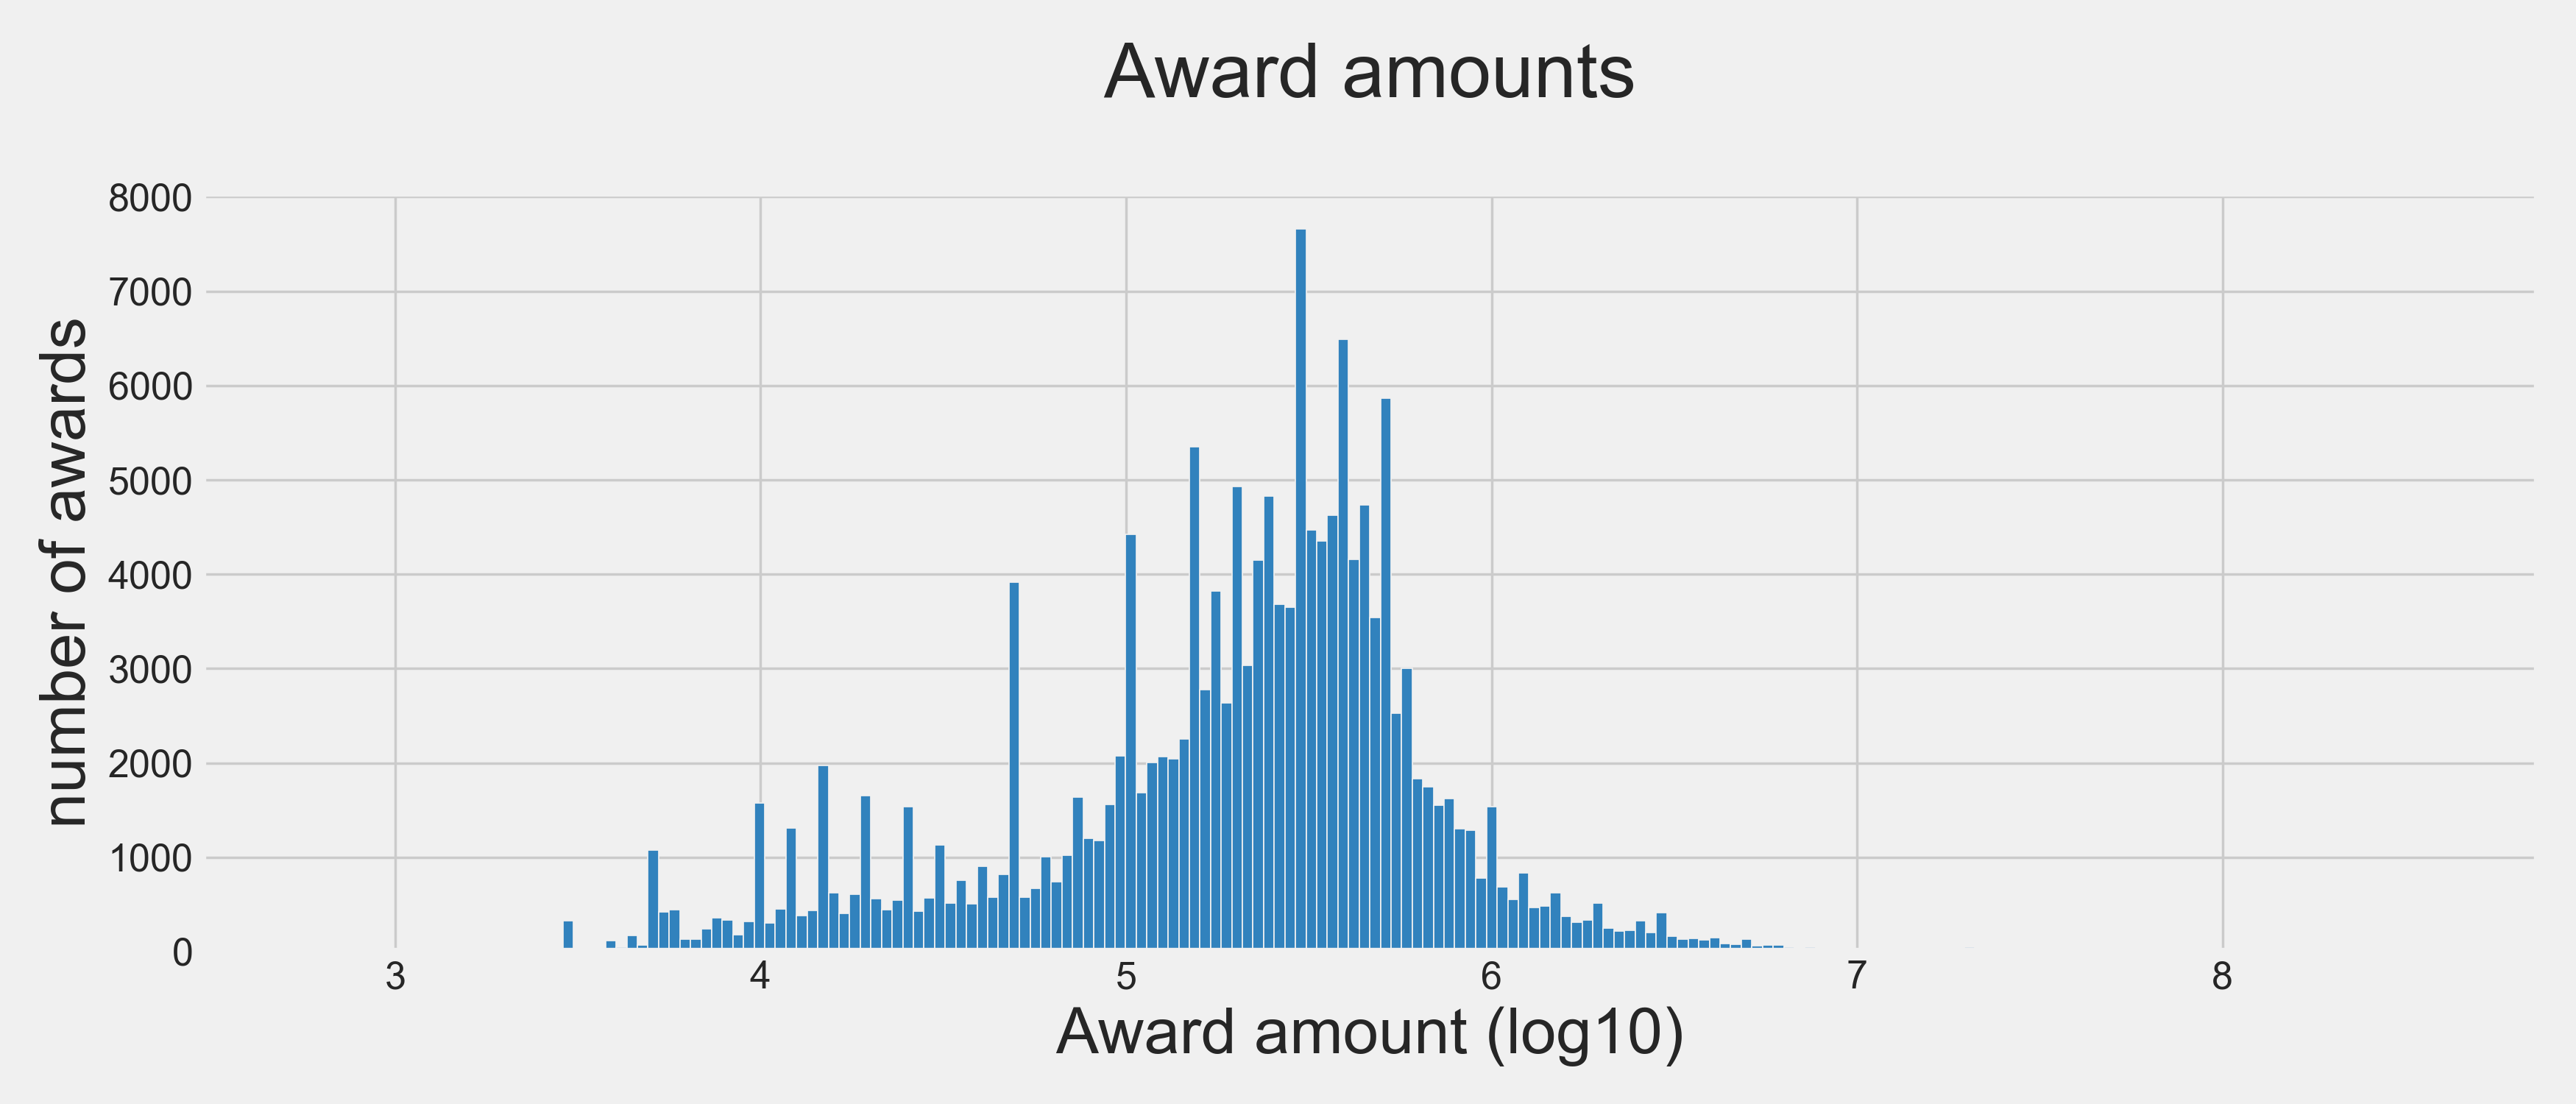
\includegraphics[width=\textwidth]{hist}

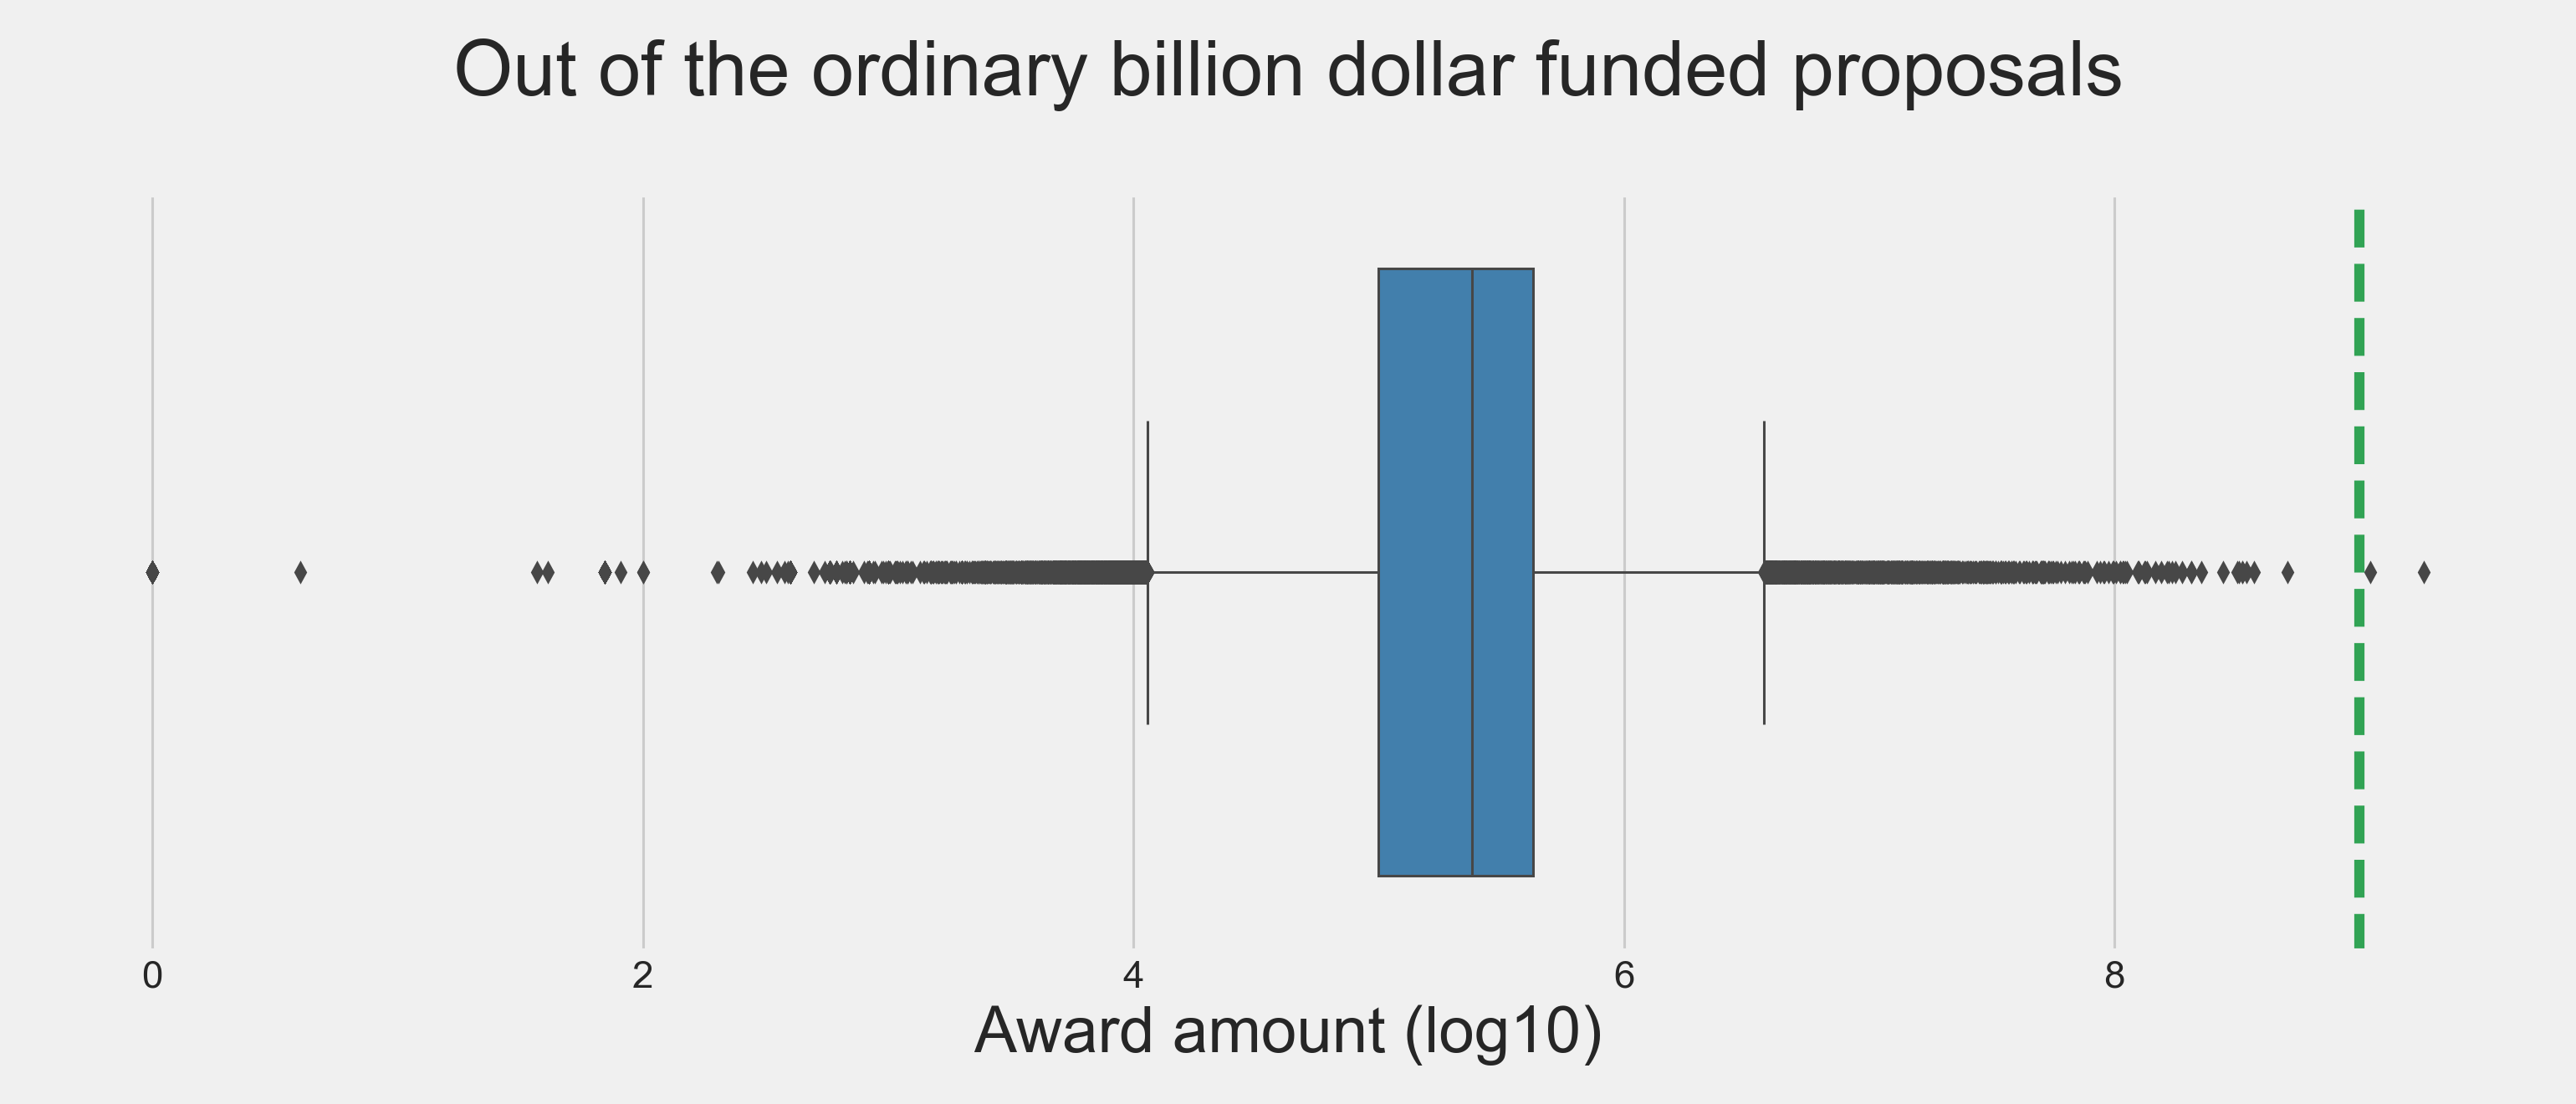
\includegraphics[width=\textwidth]{boxplot}

 \textbf{{Funding overtime} }
 
Looking at the funding trend between 2000 and 2018 shows, that in general, funding has increased over time, with the largest funded projects being awarded in 2011. There was a deep decline in 2006, which could be partially explained by the budget cut suffered by the NSF for Fiscal year 2005 as it had to operated at lower levels than 2004, affecting research directorates and programs' (NSF, 2004). Budget came back to normal levels after 2006, which is seen by the renewed increased in projects funded.

The figure below shows how the number of project funded each year has increased from 9 projects in 1999 to over 12,000 in 2016, with a sharp decline in 2006,  which coincides with budget cut shown in the previous graph.

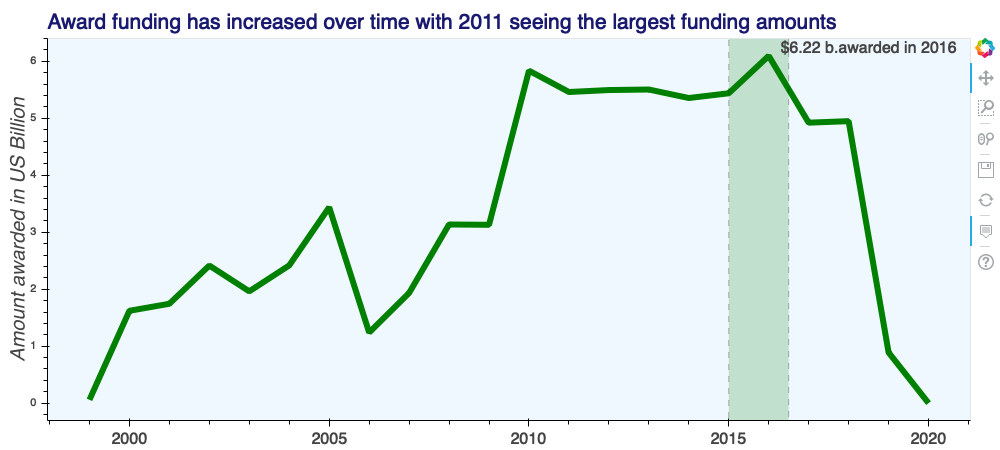
\includegraphics[width=\textwidth]{fundingovertime}

 \textbf{{Number of funded projects have also increased}}
 
Although the number of funding improved overtime, it didn't necessarily mean that the number of projects increased, as some project may receive more or less funding. A trend line of the number of projects, however, indicated that in fact the number of project also increased.

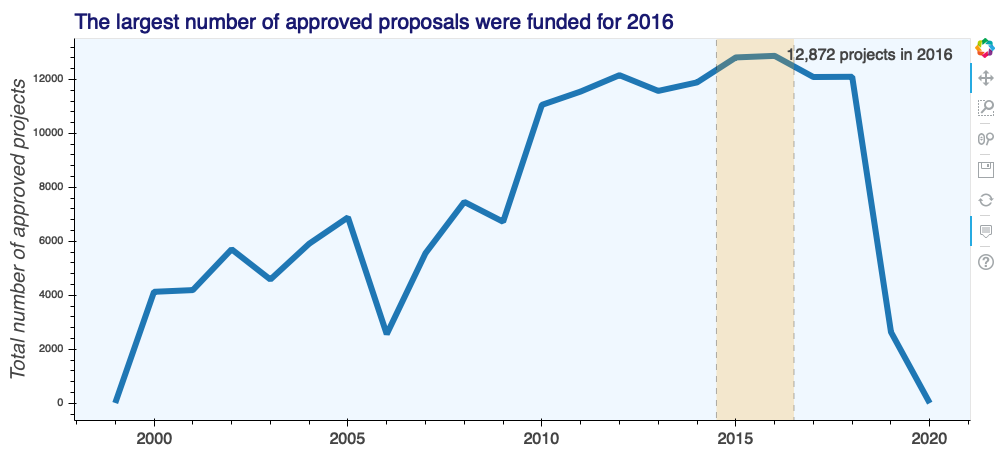
\includegraphics[width=\textwidth]{projectsovertime}

\subsection{Directorate with largest number of approved projects}

The NSF provides research and project funding 'for all fields of fundamental science and engineering, except for medical sciences' (NSF) through its directorates. Each directorate has an area of specialization, which will support specific areas of research. The first step in understanding funding patterns is to understand how many unique directorates there are and which one funds the most number of projects.
 
A visual representation of the number or projects by directorate, showed that the  \textbf{\emph{Directorate for mathematical and physical science}} has funded the largest number of projects from 2000-2018.  It has awarded since 1999 over (\$)370 million across 34,000 projects. The second largest number of projects were funded by the directorate of engineering, spending over \$46 million on 31,513 projects. The figure below shows the top 5 directorates when it comes to project funding.
 
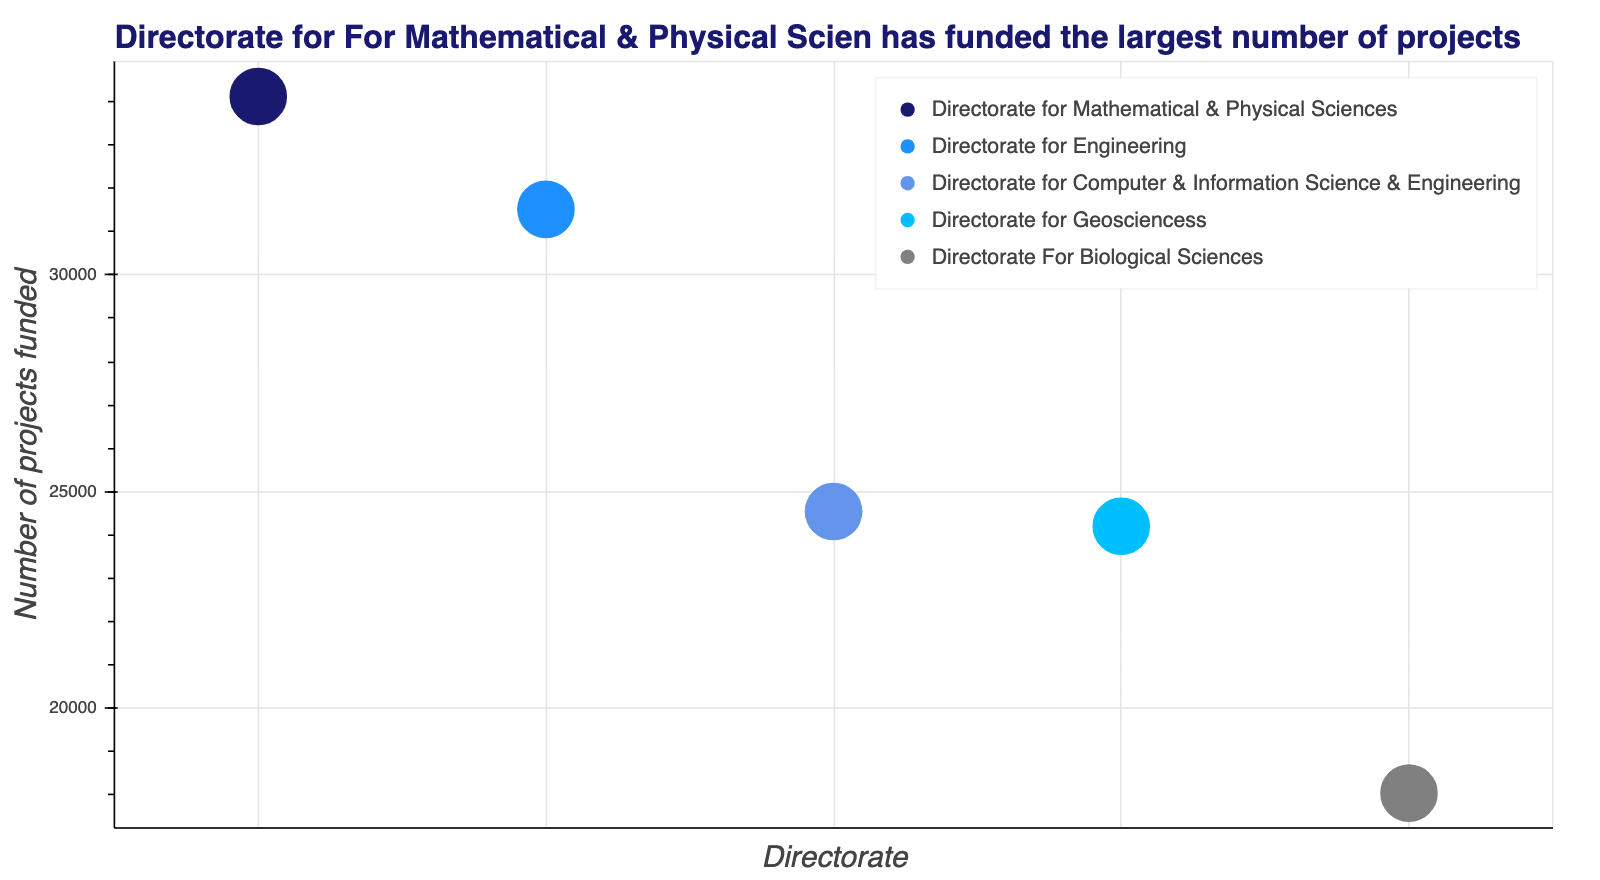
\includegraphics[width=\textwidth]{awardsperdir}
 
\subsection{Grant duration}
 
In order to make a fair comparison on the awarded amount among proposals, the grant duration was controlled by dividing the number of days between expiration and effective day by the awarded amount. This gave the daily awarded amount.

On average, the number of days between the effective and expiration date of funding was  1,180 days. 50\% of projects lasted at least 3 years and the maximum was a project that lasted over 11 years and received over a billion dollars in funding. The average amount awarded per day was \$339.39.
 
 \subsection{Semantics and language patterns}
 
Writing financial requests is not an easy task. The author has a limited amount of time and space to get her point across before the reader loses interest. Thus, a good proposal needs to have enough detail to ensure the abstract is informative, addressing the impact and feasibility of the project, but also clear and to the point so the reviewer can understand the what, when and why of the proposal in the first few minutes.

One of the assumptions of the research is that complex abstracts, those using more words per sentence and longer than average words, tend to have lower funding as they would be fairly difficult to understand. 

One of the reasons to include the flesch reading ease score as part of the predictive attributes, is that the score measures the clarity and ease of read of a text. A lower the score, means that the text is more difficult to read.

Therefore, even though proposals are reviewed by subject matter experts, the hypothesis is that abstracts that are easy to understand will be more appealing to the reviewers as they will have to spend less time trying to understand the point of the writer or the project.

\begin{center}
 \begin{tabular}{|c | c|} 
 \hline
 Score & Description\\
 \hline\hline    
90 – 100  & easily understood by an average 11-year old student \\
60 – 70 & easily understood by 13-15-year-old students\\
0 – 30& best understood by university graduates\\
 \hline
\end{tabular}
\end{center}

\vspace{5mm}

Hence,  \textbf{\emph{the hypothesis is that although many grant proposals deal with highly technical terms and in general the reviewers are subject matter experts, writing in plain English, using shorter sentences, and less unnecessary adverbs,  will lead to greater funding.}}

\vspace{5mm}
The text analysis was done using a combination of NLTK, SpaCy, and LDA (latent Dirichlet Allocation). NLTK and SpaCy were used to analyze the structure of the text, total number of words, words per sentence, average word length, lexical complexity, the flesch reading ease score, and the number of adverbs used. LDA was used for topic modeling.

 \textbf{\emph{Word count } }
 
The word count for each abstract included only the number of words without punctuation. On average, abstracts had 334 words with a standard deviation of 132 words and 80\% of abstracts having 450 words or less. 

Since abstracts are only submitted once a proposal is being considered to receive funding, the average length shows abstracts are about 30 lines of text, which coincides with the maximum number of lines for project abstracts for the National Institutes of Health, another U.S. government agency which provides vast biomedical funding. Hence, abstracts seem to be in line with other government standards.

The average number of unique words per abstract is 179 words with a standard deviation of 56 words. This shows that in general abstracts tend to avoid redundancy.

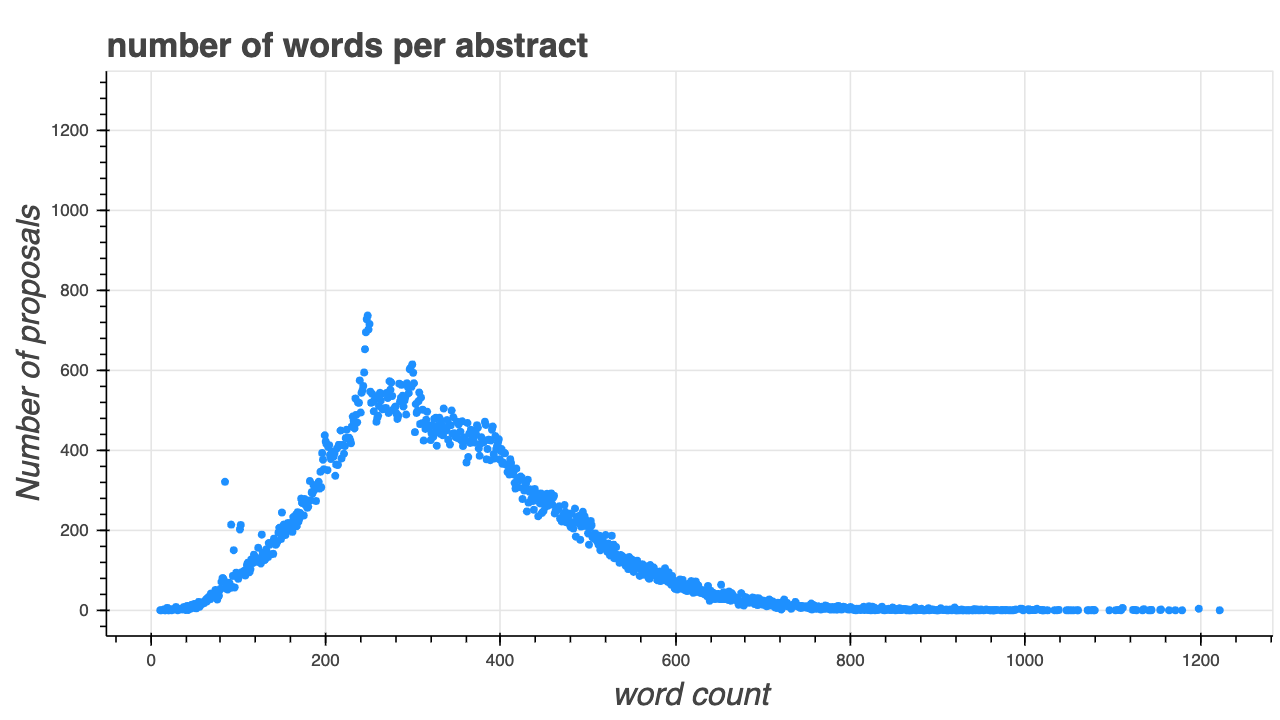
\includegraphics[width=\textwidth]{totalwordcount}

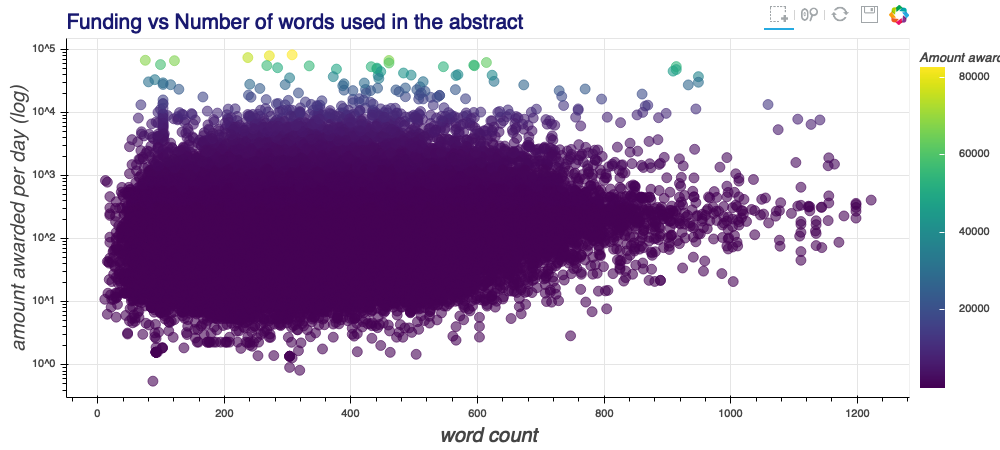
\includegraphics[width=\textwidth]{wordawards}

\textbf{\emph{unique words}}

The average number of unique words per abstract is 179 words with a standard deviation of 56 words. This shows that in general abstracts tend to avoid redundancy.

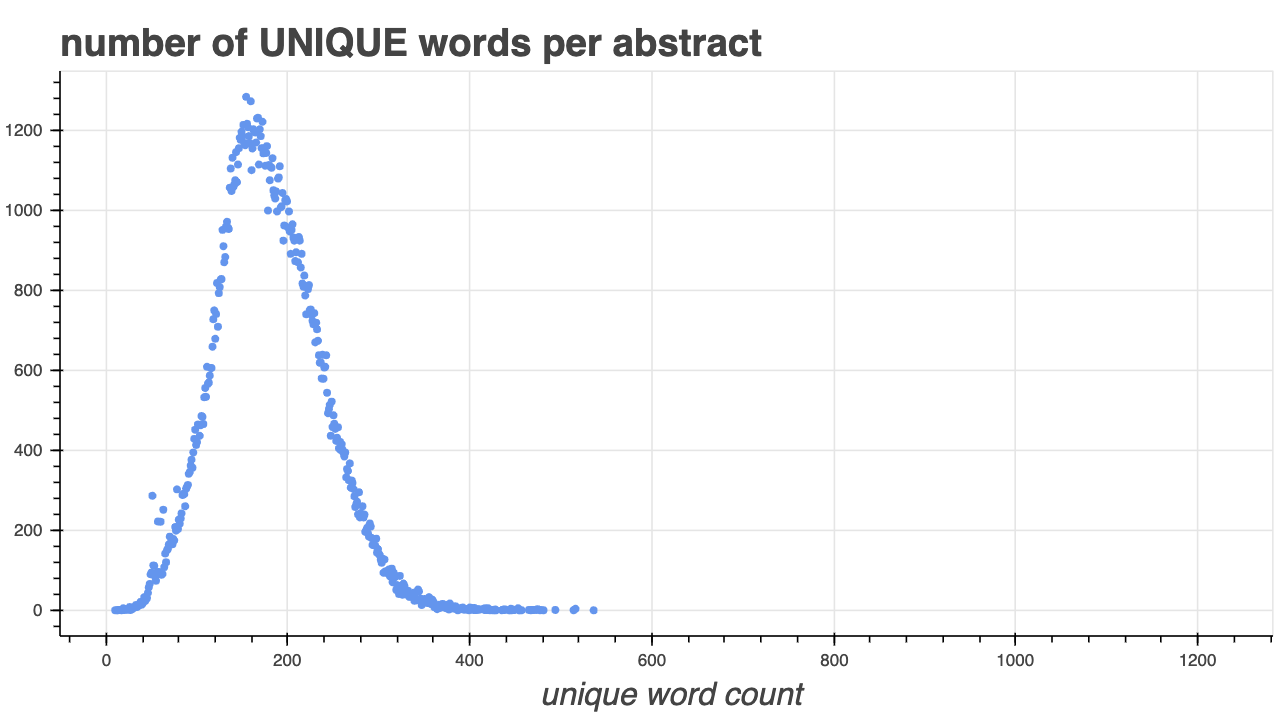
\includegraphics[width=\textwidth]{uniquewords}

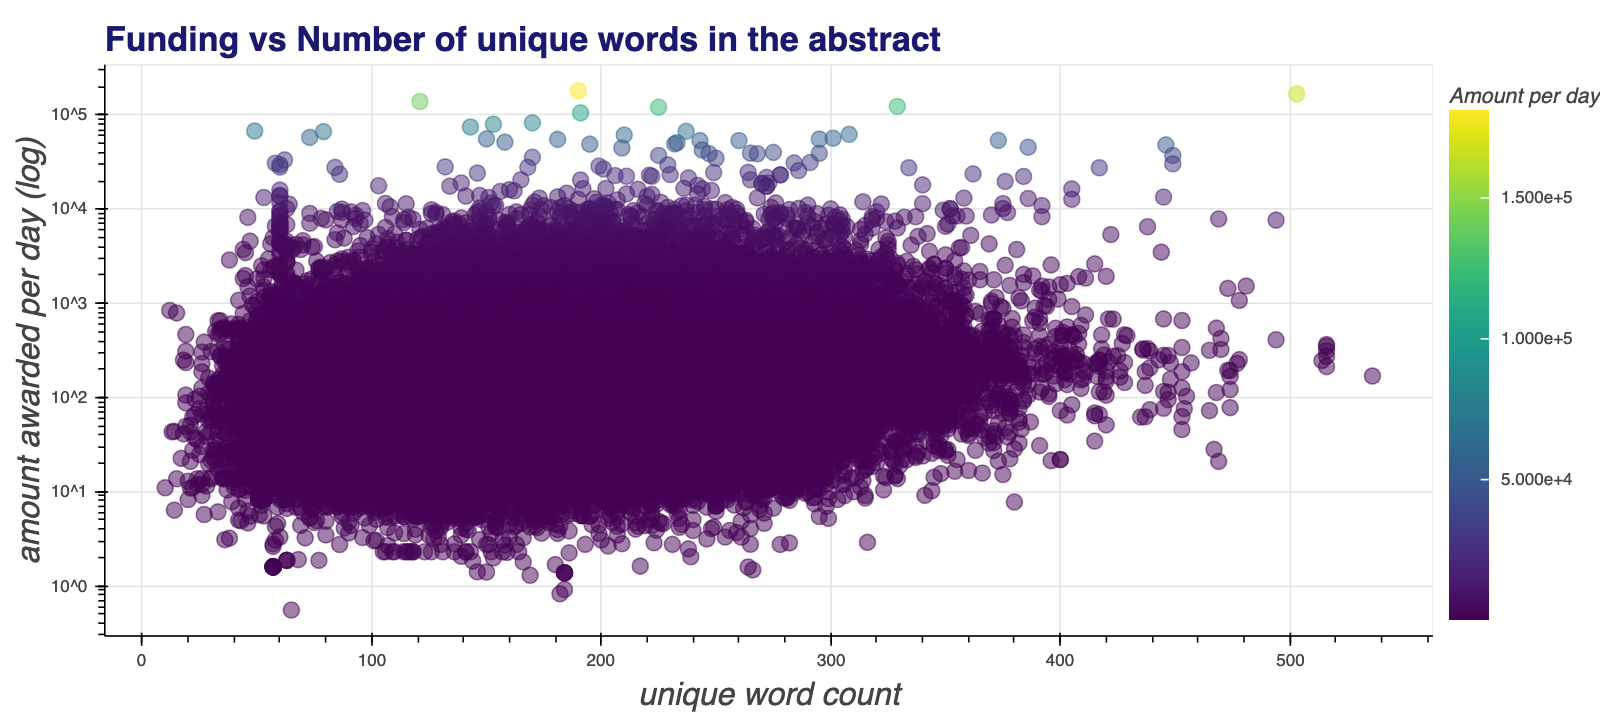
\includegraphics[width=\textwidth]{uniquewordsawards}

\textbf{\emph{Empirical Cumulative Distribution Function}}

A visual representation of the ECDF for total words used vs. unique words shows that 80\% of abstracts use at least 200 unique words.

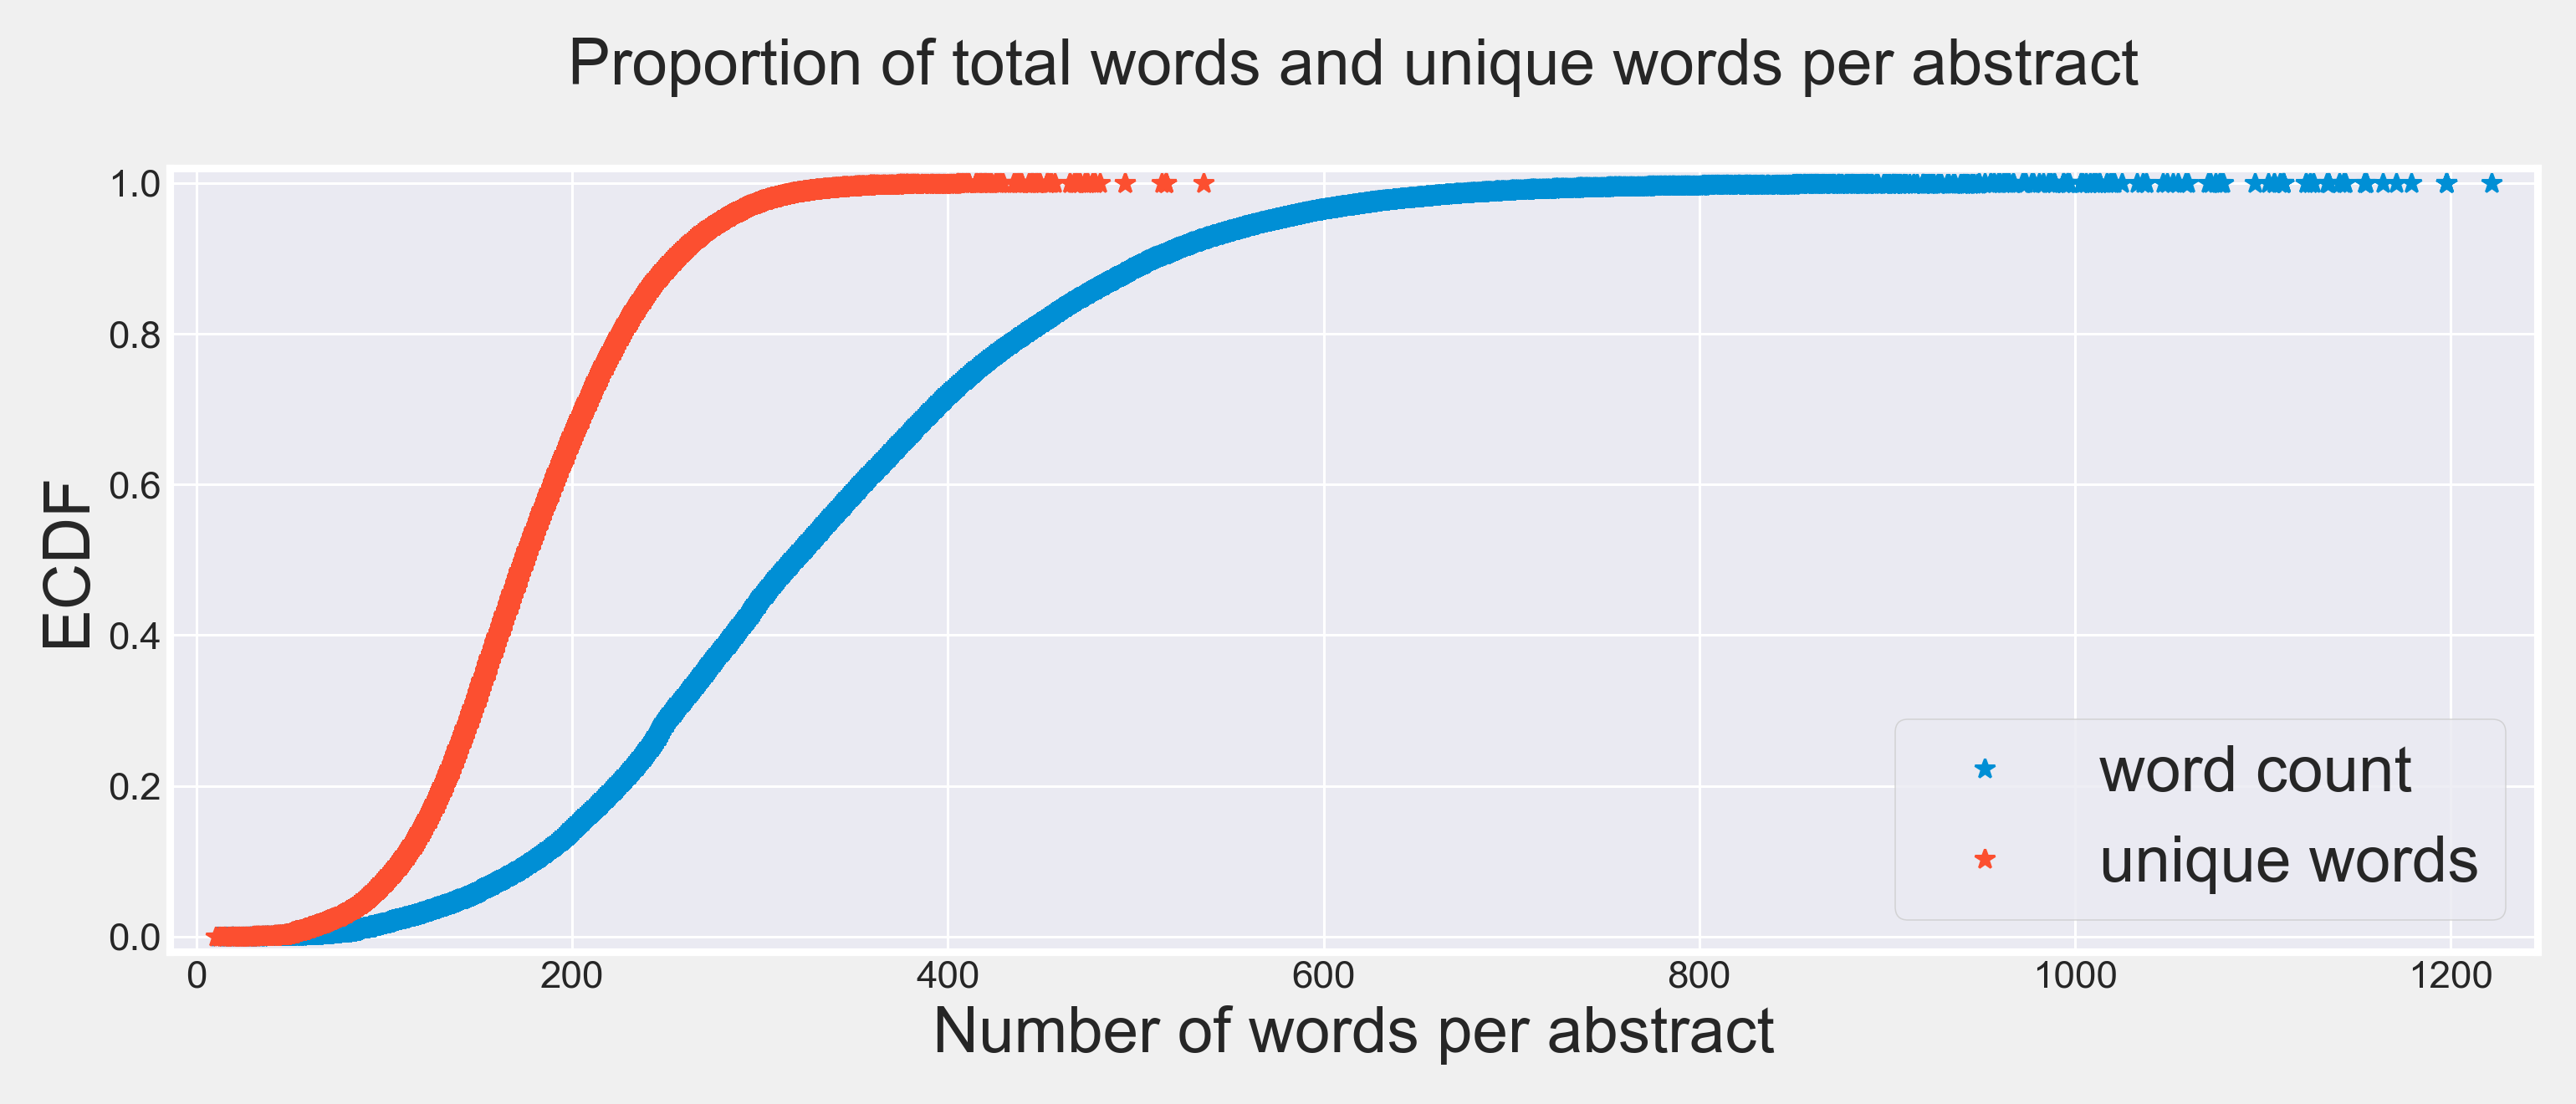
\includegraphics[width=\textwidth]{ecdf}

\textbf{\emph{Length of the abstract}}

The length of the abstract, which considers all characters not just words, tells us how lengthy the project descriptions are and whether this can have an impact on the aid received.

The scatter plot shows that as the length increases, the award amount tends to increase. This would suggest that in general, longer proposals with more distinct words tend to obtain more funding than shorter ones. A possible reason is that detailed proposals that use clear and unique words are perceived as having a clearer and specific idea on why the project is important and how the funds will be used.

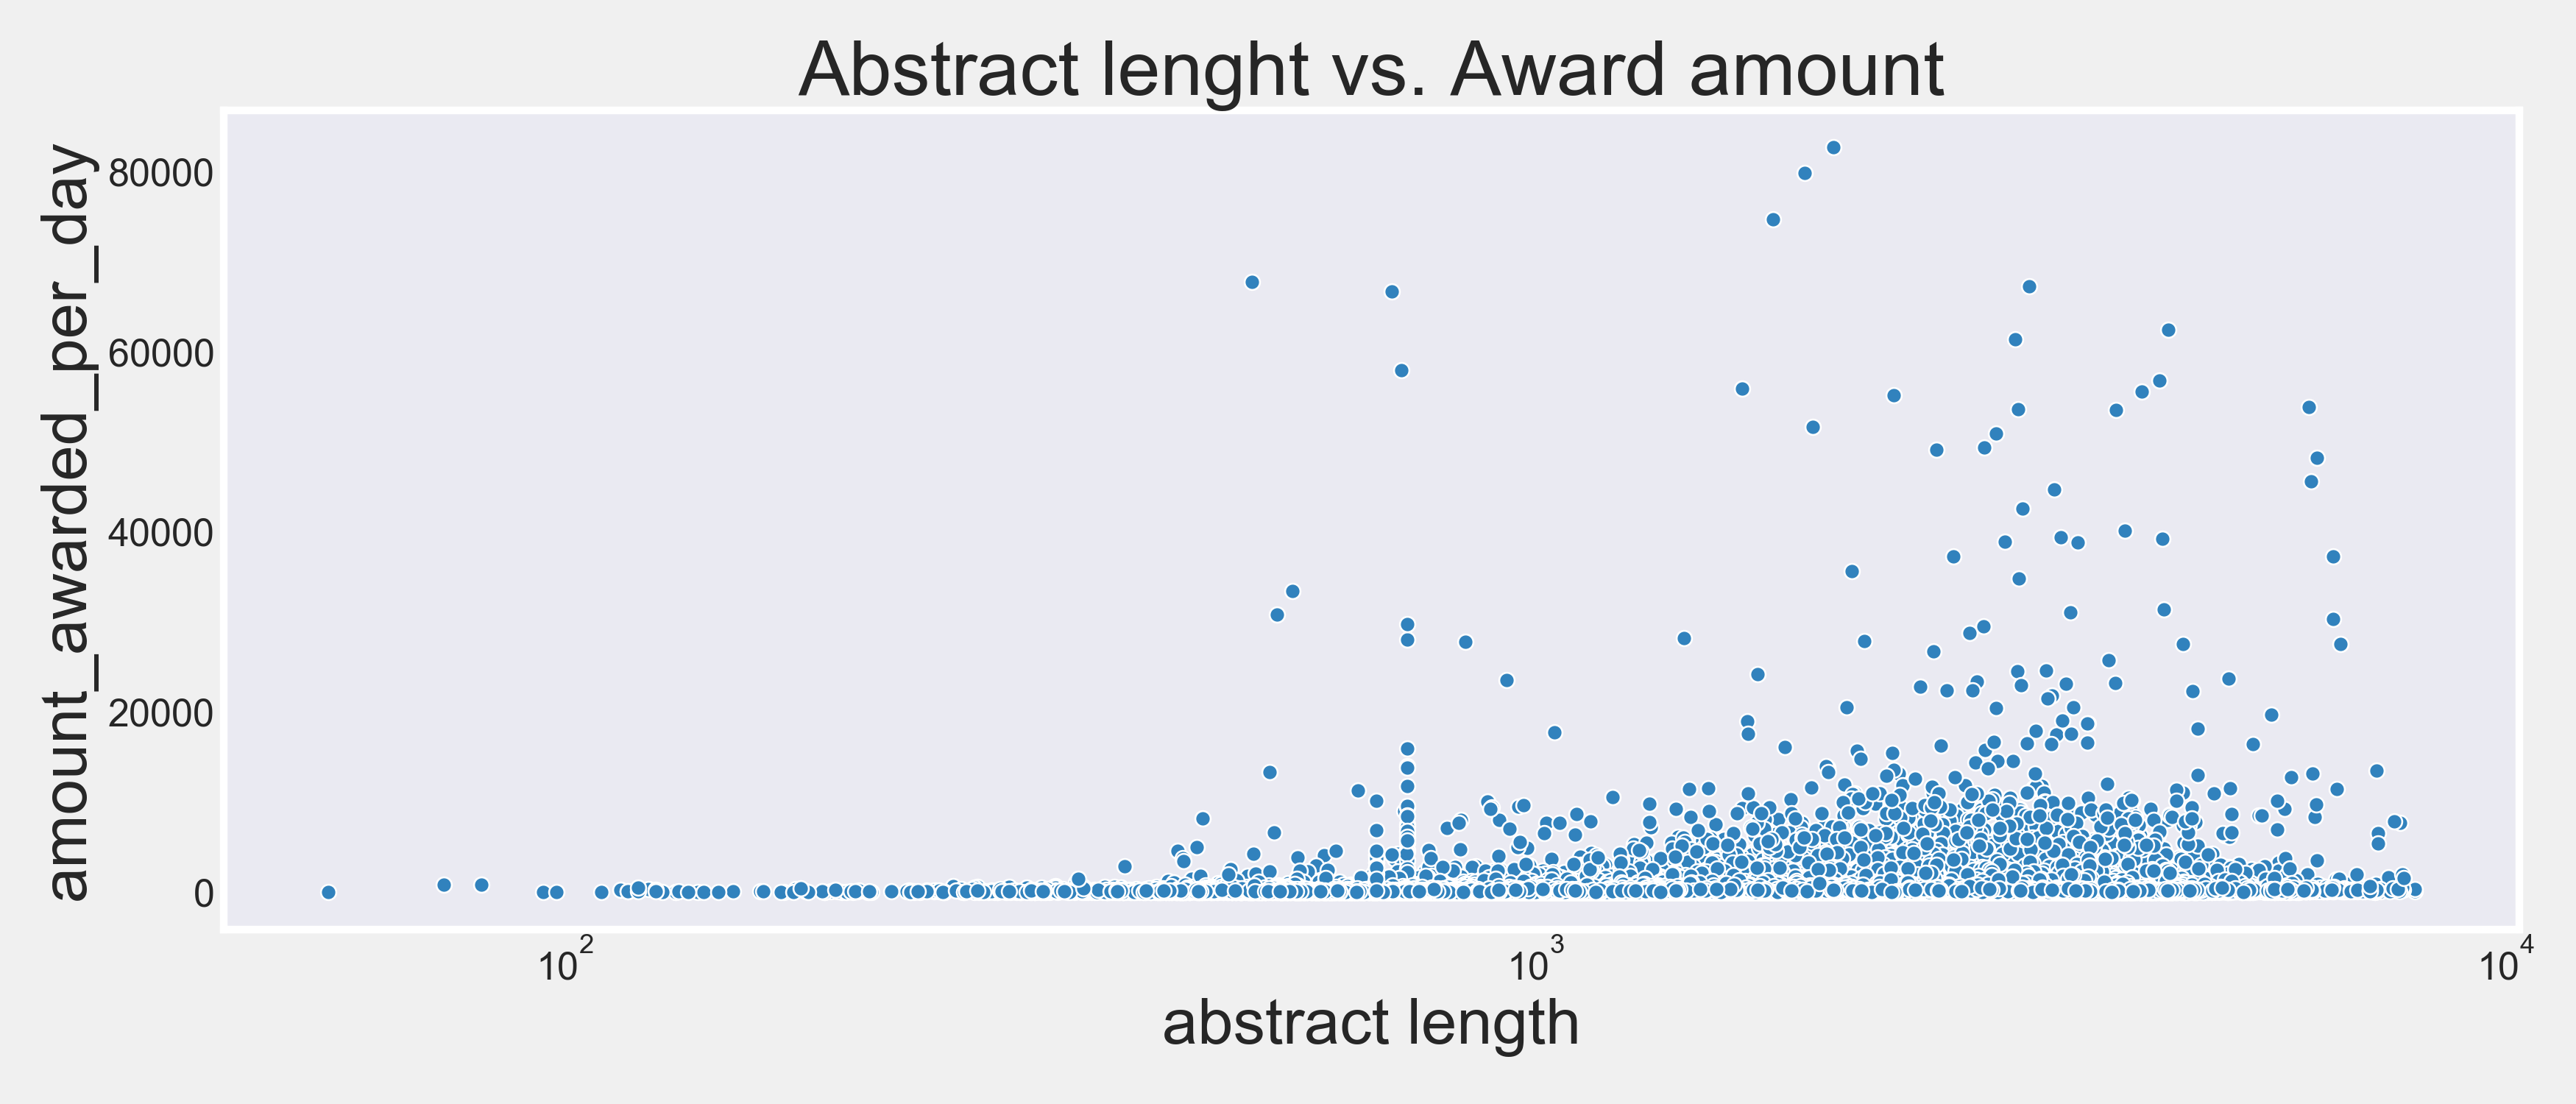
\includegraphics[width=\textwidth]{abstractlengthscatterplot}

\break
\textbf{\emph{Shorter sentences improve comprehension} }
 
Easy to understand sentence have in general between 15 - 20 words. More than that and the reader tends to get lost. The average number of sentences per abstract is 30 words, making sentences longer than average and harder to understand. Even though many of the reviewers are subject matter experts, several studies have shown that sentences with '29 words or longer are very difficult to understand' (GovUK). This not only hurts comprehension, but it slows down the review process.

\textbf{\emph{Writing style} } 

One of the ways to determine a writer's style is by the number of adverbs used. Although adverbs are an important part of the speech, too many can suggest ambiguity and even a 'timid' writer, according to \href{https://www.brainpickings.org/2013/03/13/stephen-king-on-adverbs/}{Stephen King}. 
 
\textbf{\emph{Complex words} } 

The average word length per abstract is five words, indicating applicants favor common and less complex words, even when they use more words per sentence. The word length for 75\% of the abstracts is 6 words, which is in line with the average length of common words.

\textbf{\emph{Lexical complexity} } 

The lexical diversity shows the proportion of unique words from the total number of words used. On average, the number of distinct words is 56\% and 75\% of the documents use on average 60\% unique words of all the words. This shows once again, that applicants are choosing the best words to describe their projects without repeating the same 

On average, abstracts contain just 10 adverbs. Considering the average abstract length in 333 words, based on the data, abstracts are written in a  direct and assertive way. 

\textbf{\emph{Average word count per sentence}}

Easy to understand sentences have in general between 15 - 20 words. More than that and the reader tends to get lost. The average number of sentences per abstract in this data set is 30 words, making sentences longer than average and harder to understand.

Even though many of the reviewers are subject matter experts, several studies have shown that sentences with '29 words or longer are very difficult to understand' (GovUK). This not only hurts comprehension, but it slows down the review process.

\textbf{\emph{Average word length}}

The average word length per abstract is five words, indicating applicants favor common and less complex words, even when they use more words per sentence. The word length for 75\% of the abstracts is 6 words, which is in line with the average length of common words.

\textbf{\emph{Flesch reading ease score}}

The flesch reading ease score measures the clarity and ease of read of a text. A lower the score, means that the text is more difficult to read.

Therefore, even though proposals are reviewed by subject matter experts, the hypothesis is that abstracts that are easy to understand will be more appealing to the reviewers as they will have to spend less time trying to understand the point of the writer or the project. 

The plots for the abstracts' flesch score showed that that the majority of the abstracts are written for at the graduate level and intended for subject expert matters. 75\% of the abstracts have a score of 19 or less.

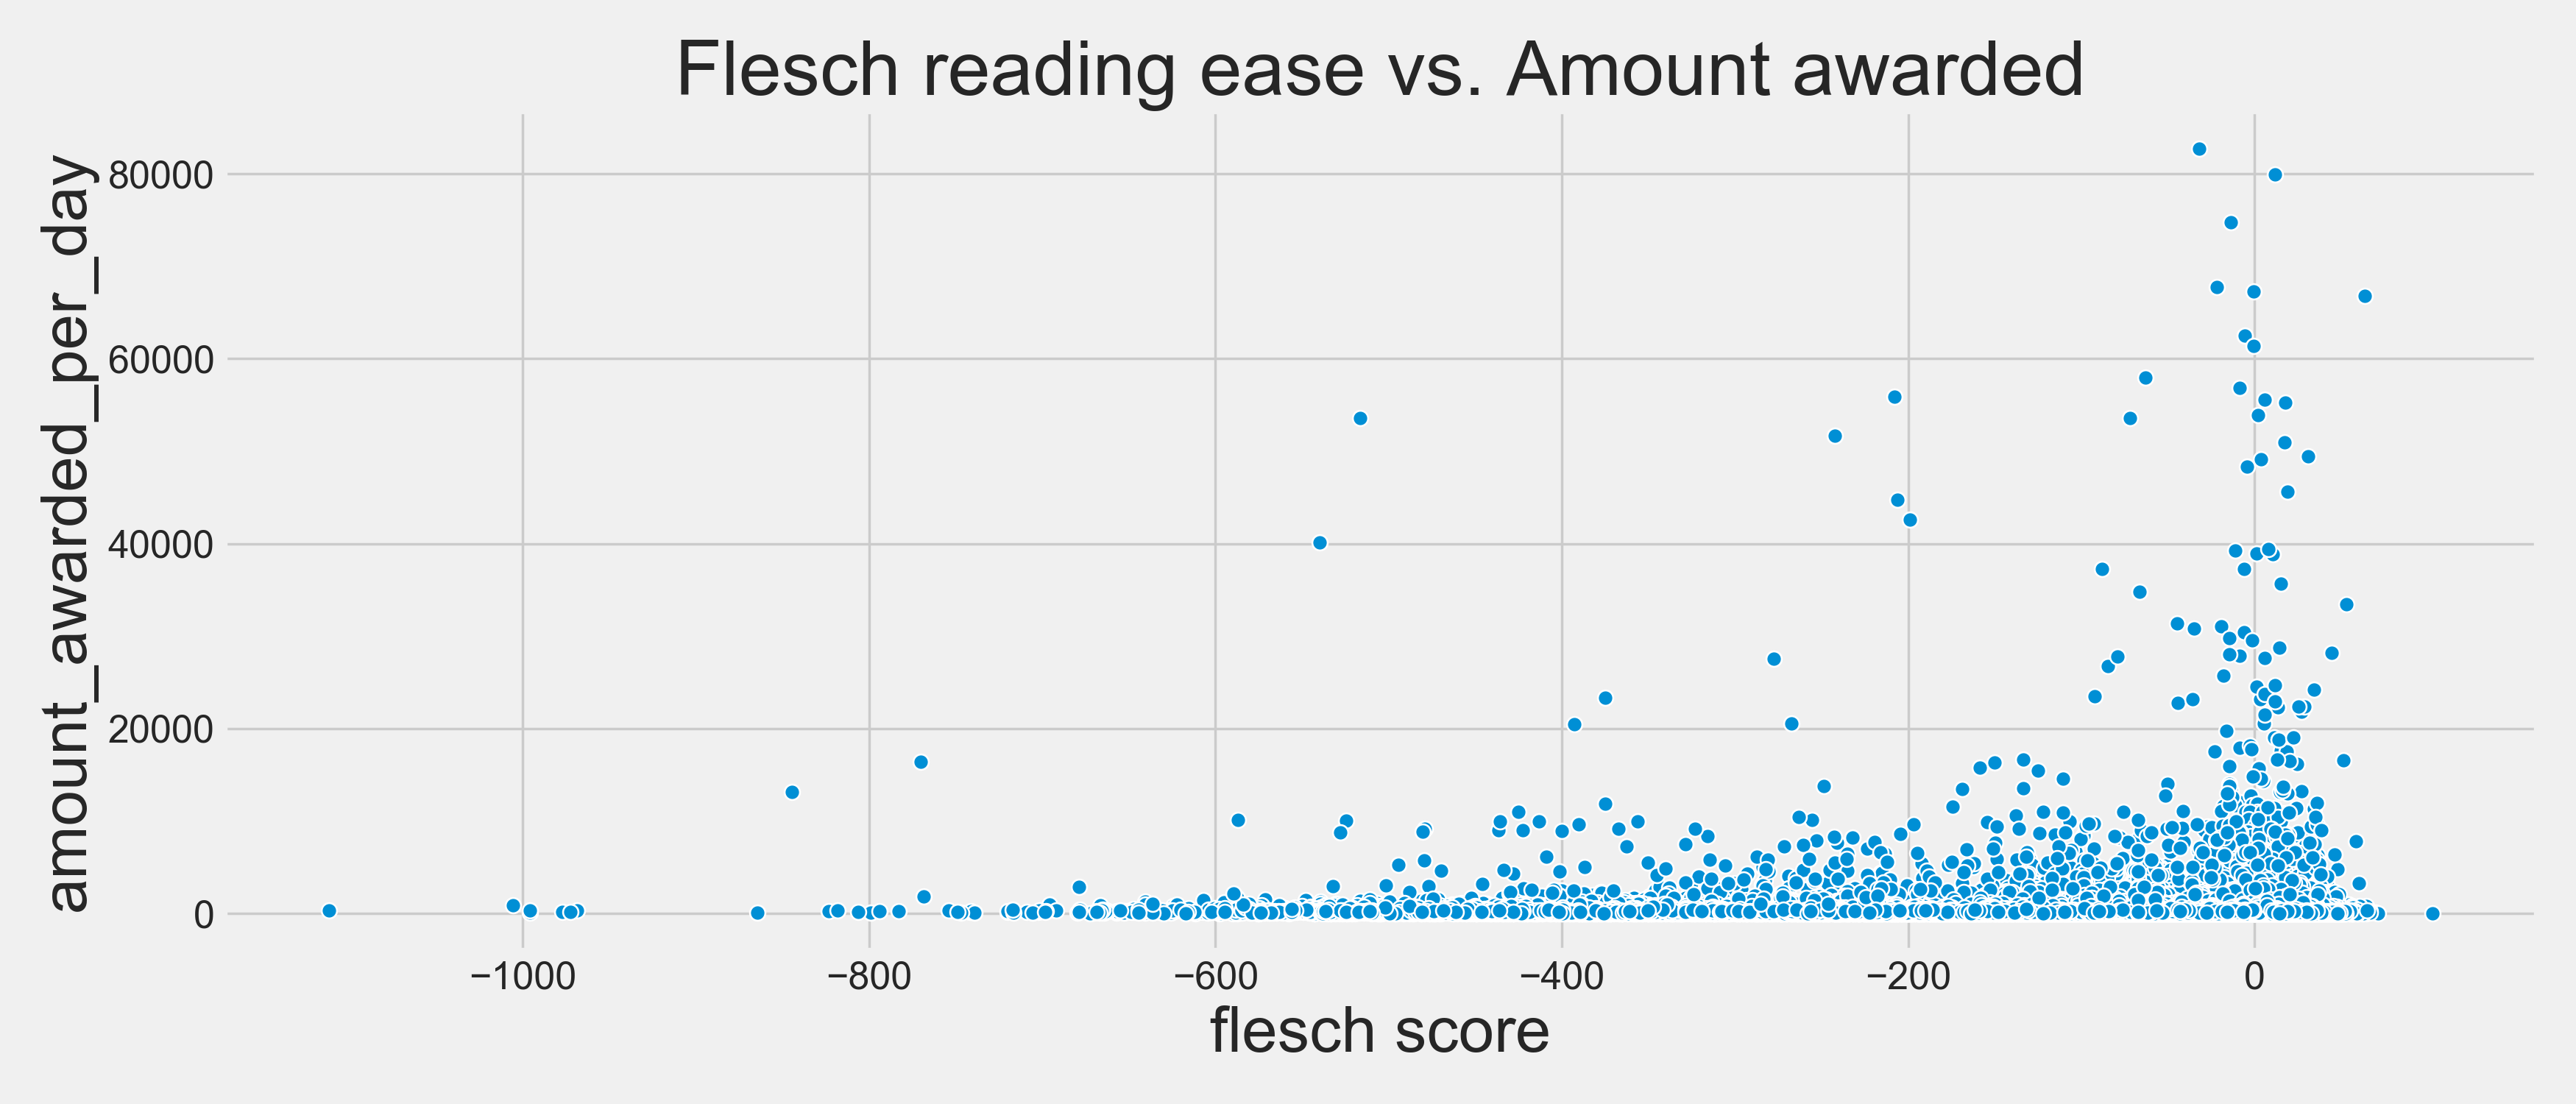
\includegraphics[width=\textwidth]{fleschscore}

 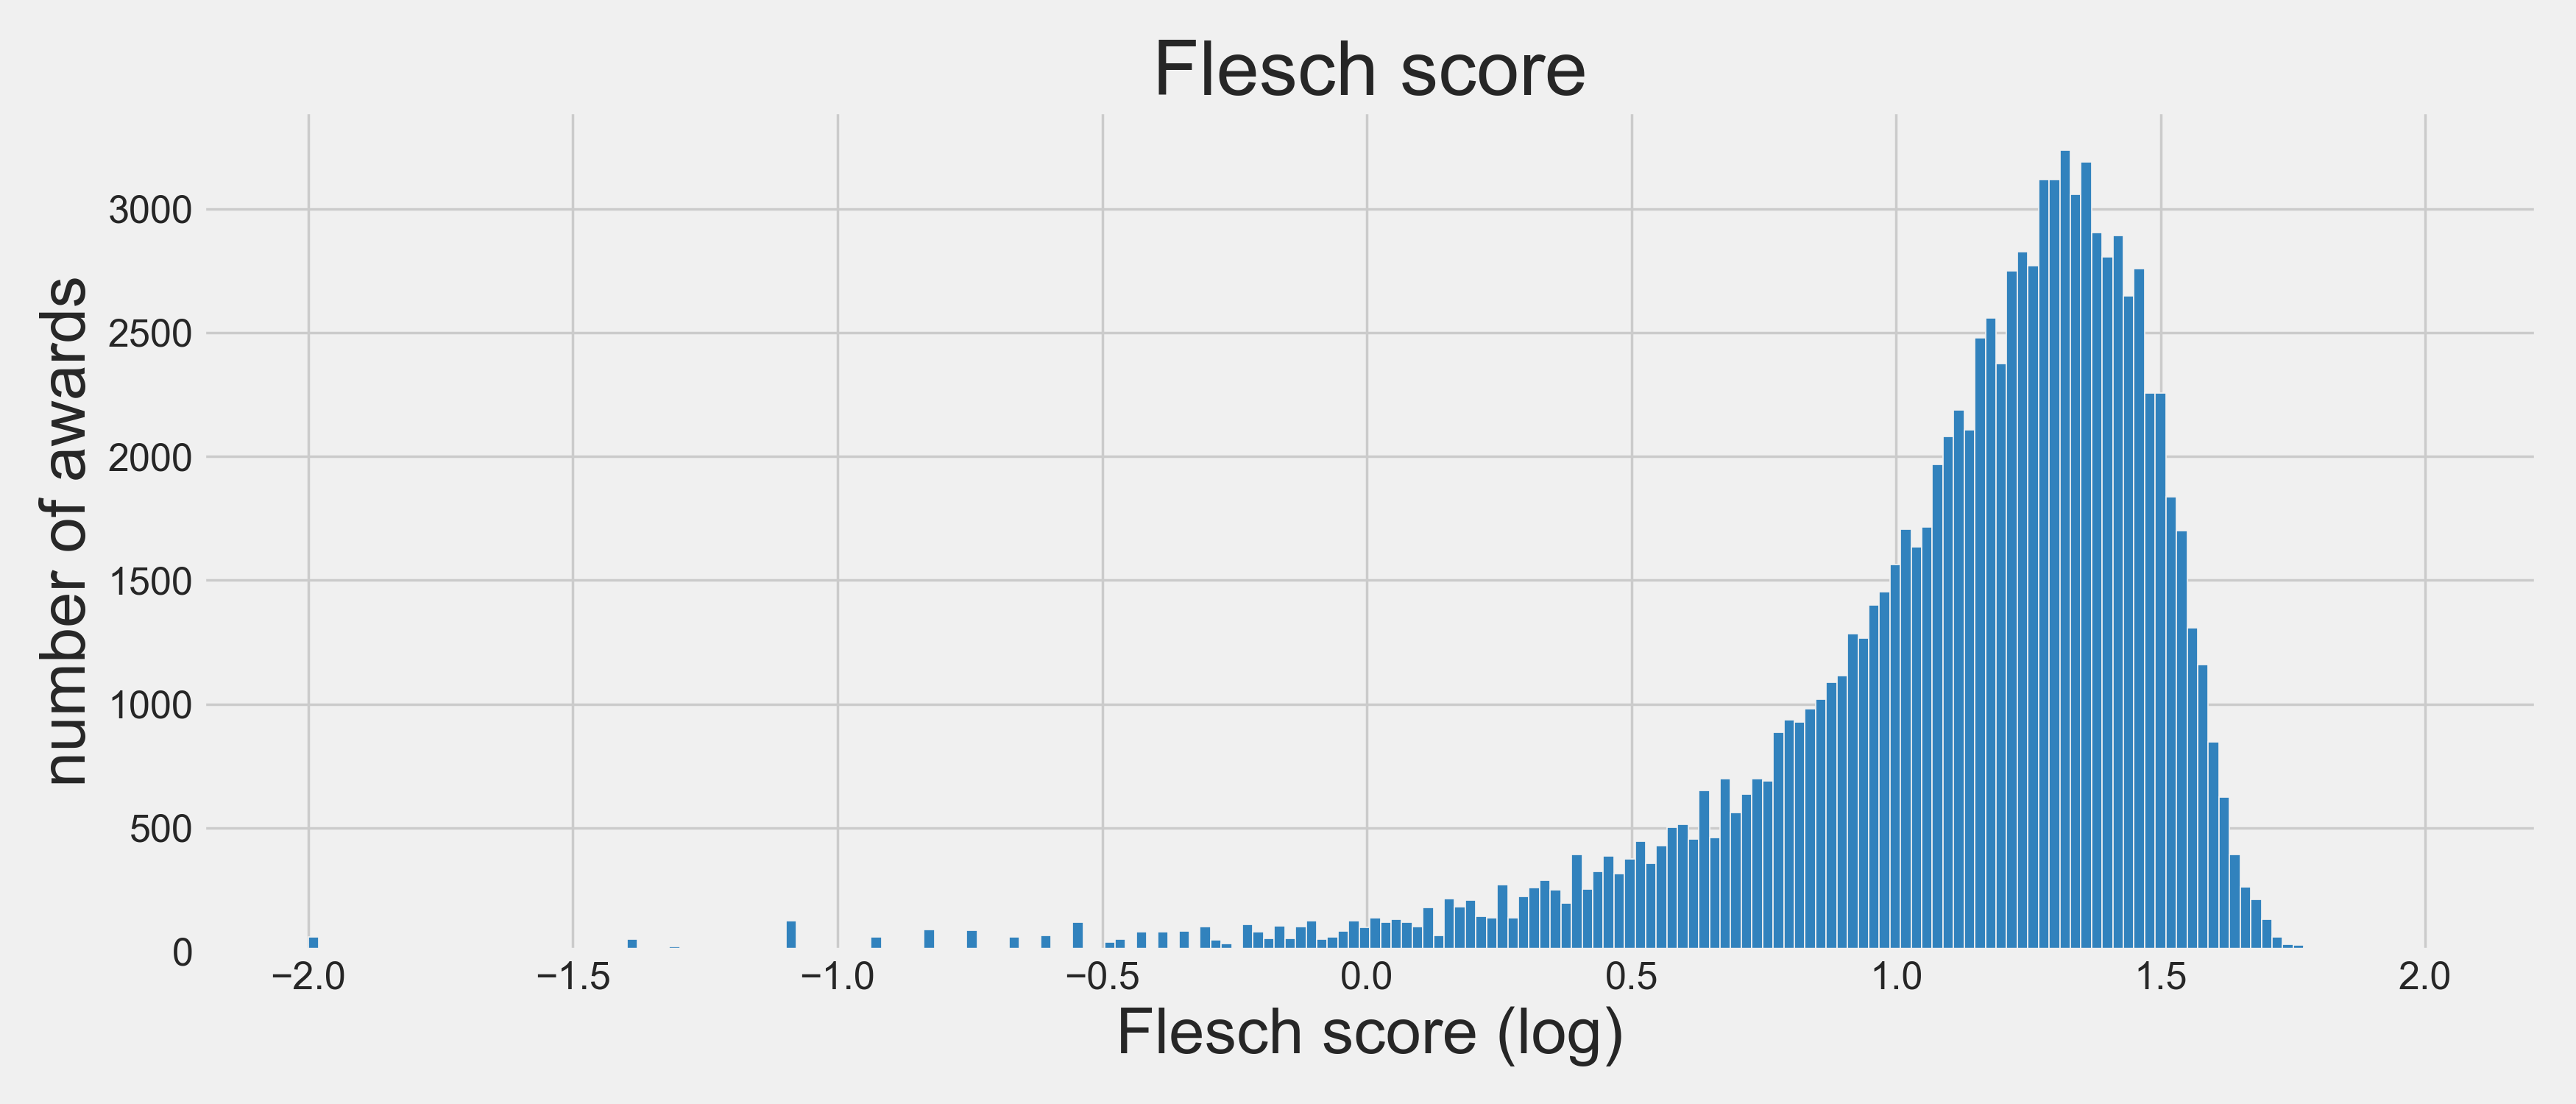
\includegraphics[width=\textwidth]{fleschscorehist}
 
 \subsection{Approved projects by gender} 
 
Once reviewers have evaluated proposals, the NSF program officer for each division reviews the proposal and makes the decision to award or deny funding. One of the questions of the project is whether gender has an effect on the number of proposals approved and the amount of money awarded.
 
Since the data provides information on the name of the NSF program officer who signed the approved proposal, a model was created to predict the gender of all program officers. Two models were tried, an NLTK classifier which used a list of 8000 common male and female names; and a naïve bayes model. 
 
Since the accuracy of the NLTK classifier was  77\% compared to just 66\% for the naïves bayes, this model was used for the entire dataset to create a new attribute that would be used in predicting the award amount.
 
One of the hypothesis is that gender may have an effect on the amount of money received by a grant. Since the only thing we have is the name of the person who signed the grant proposal, we use the first name to predict the gender and then use this attribute in the final model. Although not perfect, this can give us an insight on the grant proposal and approval process.
 
Based on the predictive model, the number of male program officers reviewing proposals outnumber women throughout the years. Although this is by no means a perfect measure of the number of women per department, it shows that there is a greater number of male reviewers. 

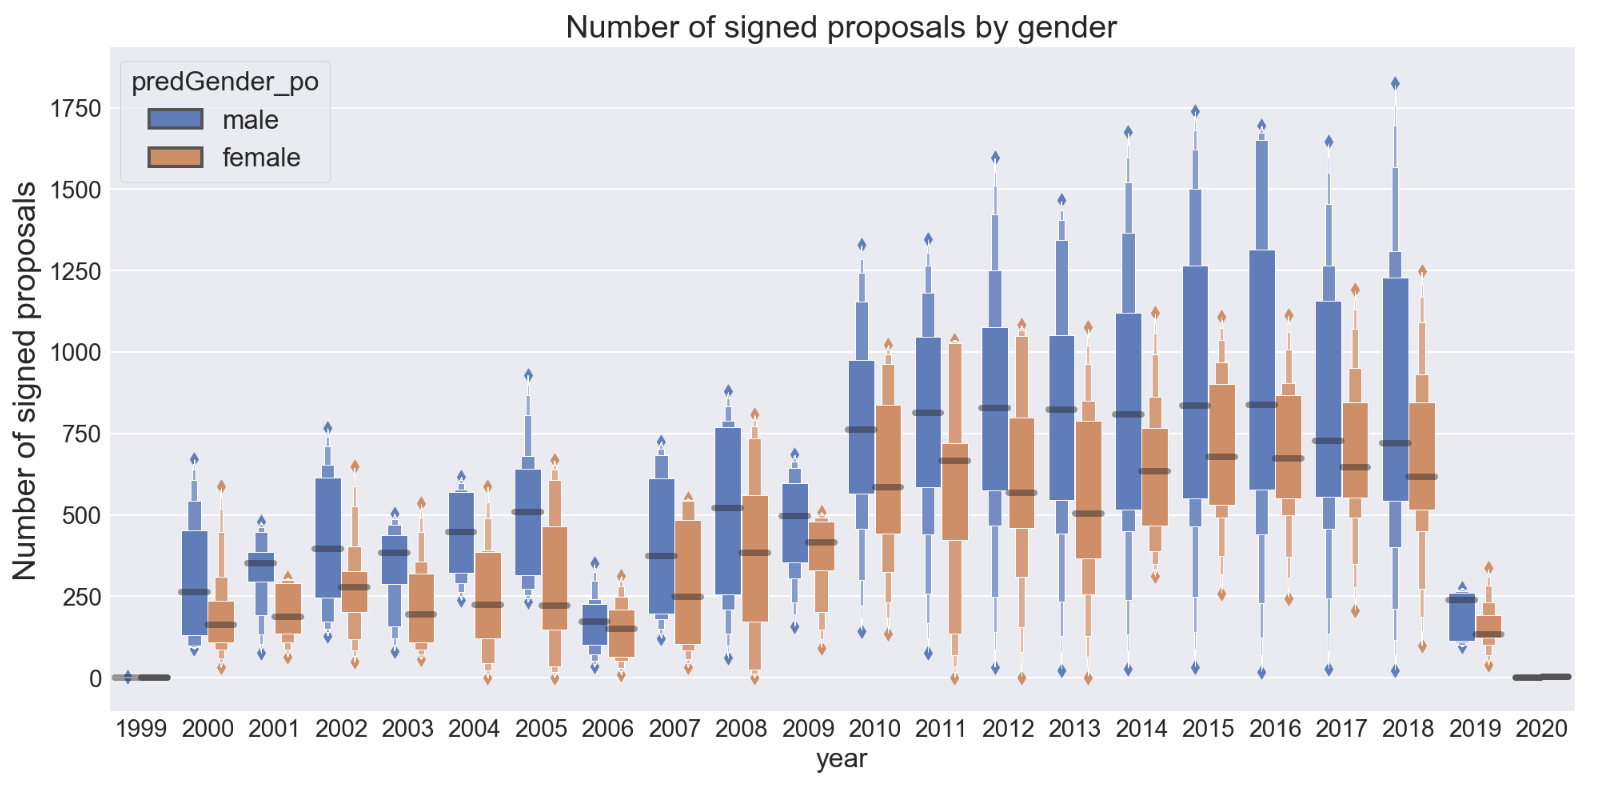
\includegraphics[width=\textwidth]{programofficergender}

 \section{{Topic modeling} }
 
In order to obtain the topic of each abstract and use it as a feature in predicting the amount of funded received, the abstract text was analyzed and summarized using Latent Dirichlet Allocation (LDA).
 
 LDA is an unsupervised algorithm that takes the complete corpus, identifies patterns among words and selects the number of topics we ask it to find. In this case, since there are nine different NSF directorates, 10 topics were selected.
 
From the ten topics found, the model predicts that abstracts that are 'tagged' with topic 0, refer to academic scientific research.
 
 The hypothesis is that technological research tends to receive more funding compare to other areas such as biology or environmental studies.
 
 The following figures show the most relevant terms in each of the ten topics identified by the LDA model.
 
 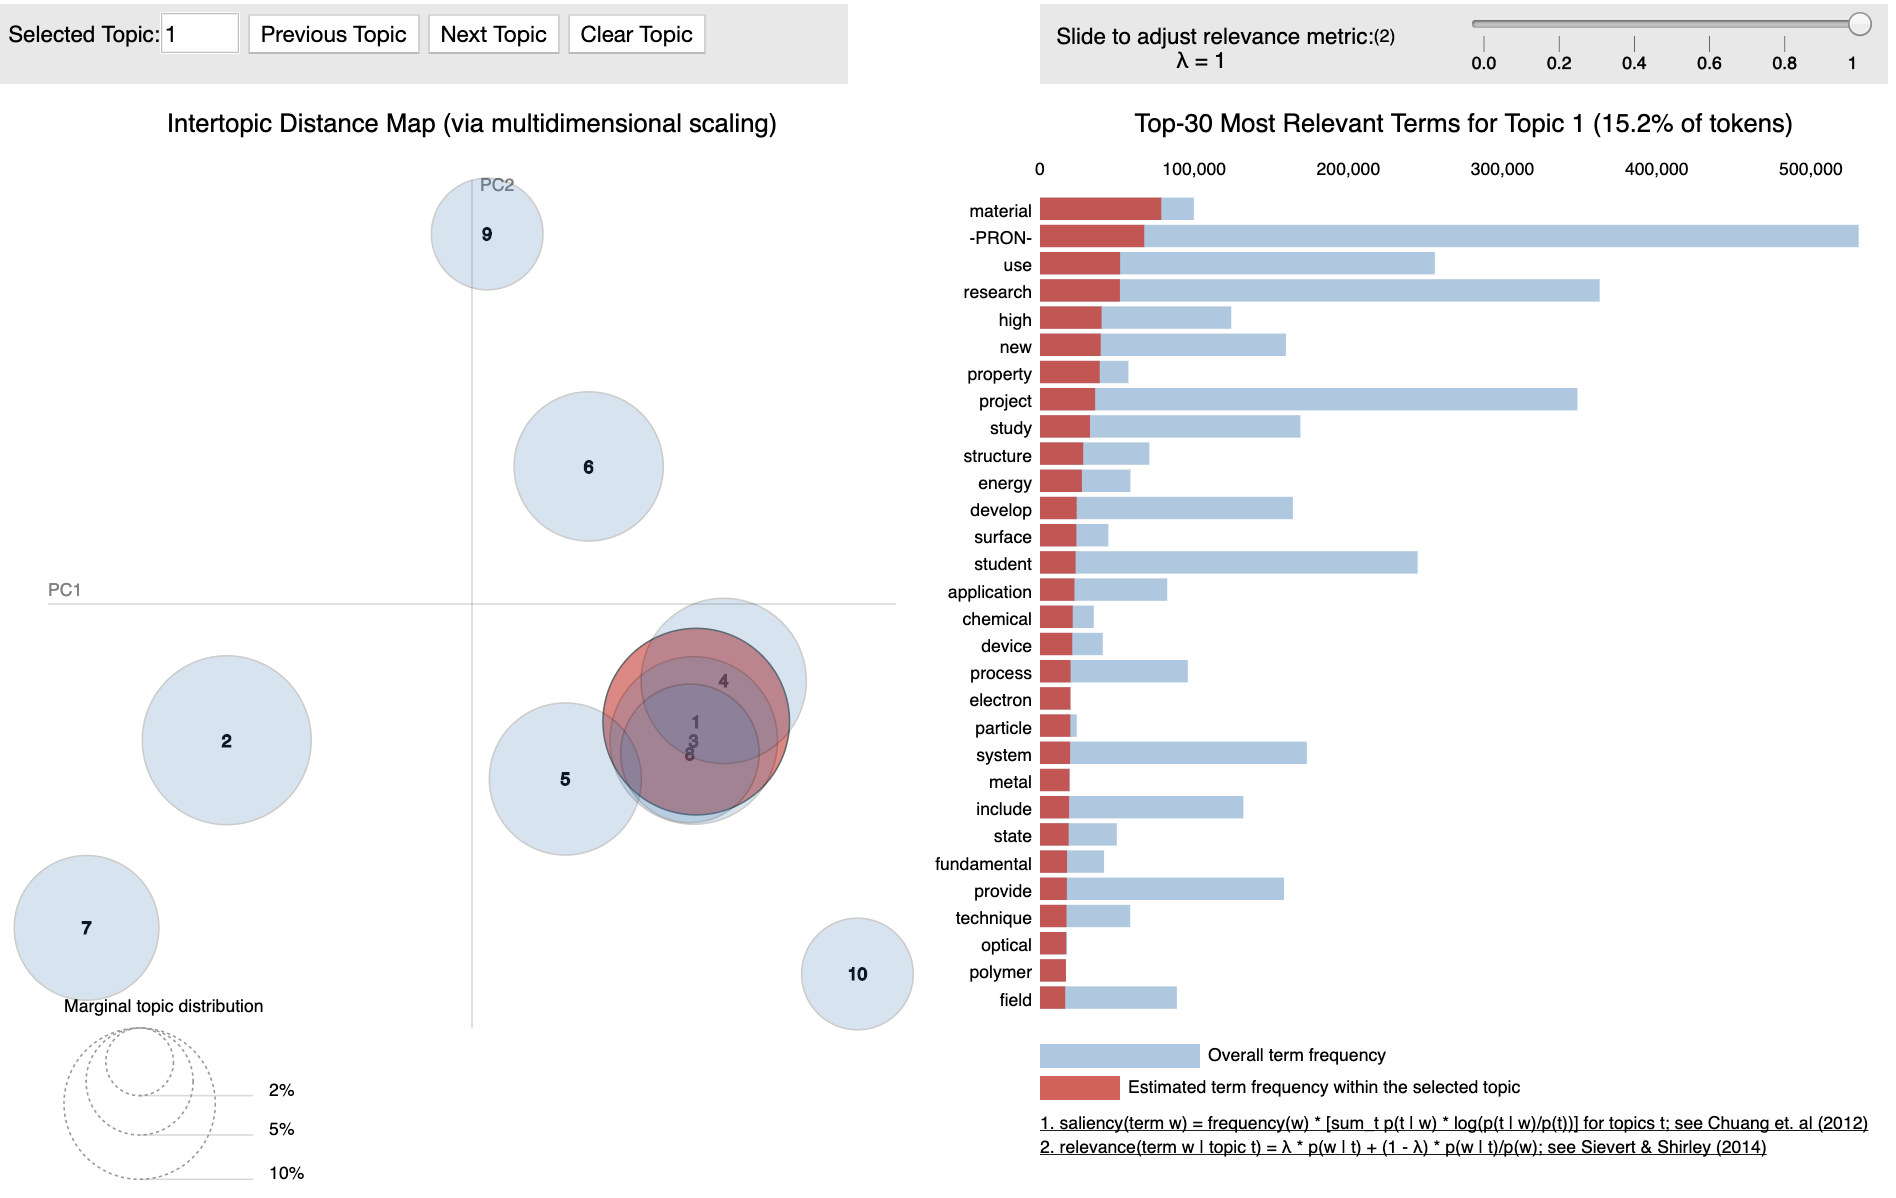
\includegraphics[width=\textwidth]{ldaVisualizationTopic1}
 
The model found that topic 1 is related to scientific research, focusing on energy and chemical reactions with words like energy and electrons.
 
 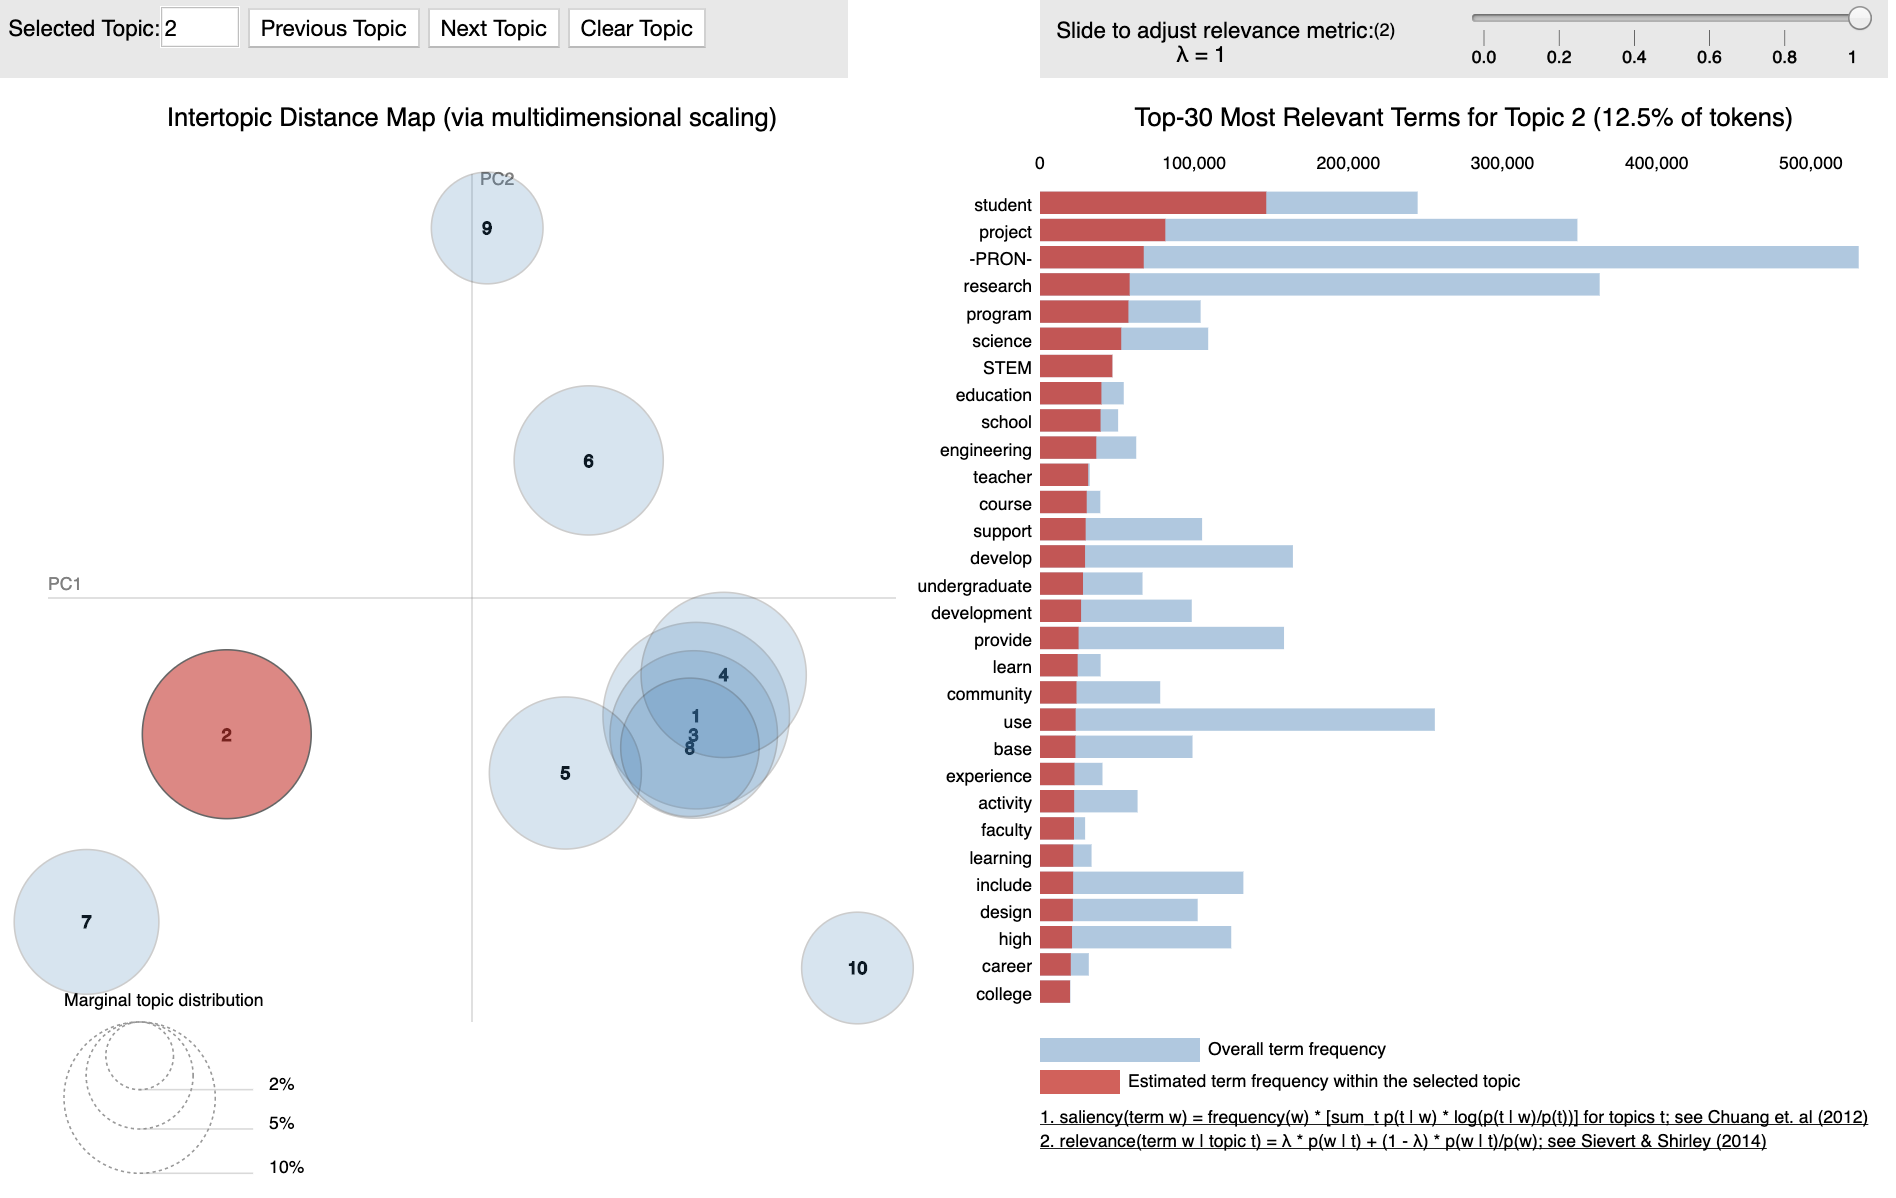
\includegraphics[width=\textwidth]{ldaVisualizationTopic2}
  
 Topic 2, centers around technology and STEM academic research, with words like  STEM, engineering, student and research.
 
  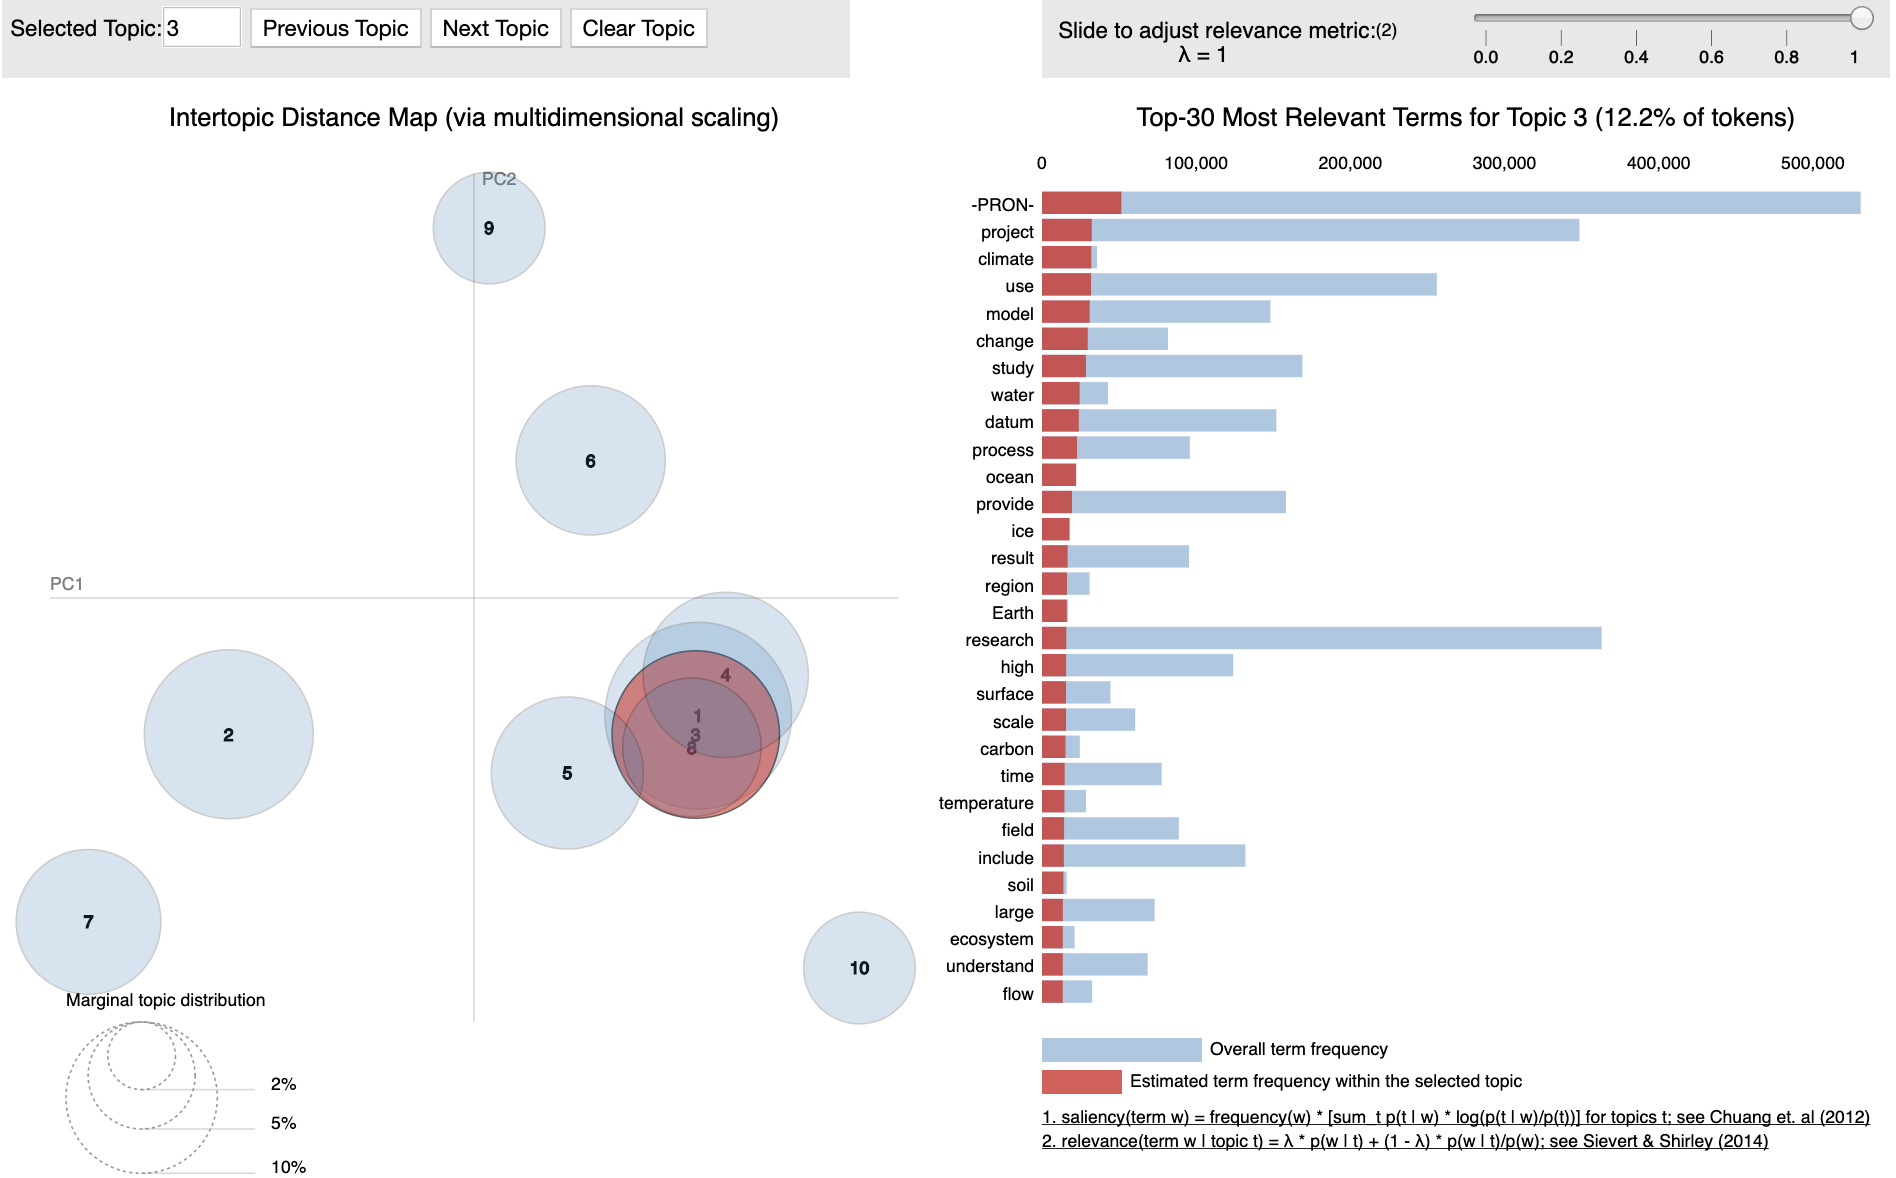
\includegraphics[width=\textwidth]{ldaVisualizationTopic3}
  
  Topic 3 focuses on the environment, with words like temperature, climate and ecosystem.
 
 \section{Predicting Award Funding} 
 
After obtaining attributes from the text analysis, the data was ready to build the model to predict the amount of funding based on text patterns using Extreme Gradient Boosting (XGBoost).

The goal of XGBoosting is to train multiple models and sequentially combine them to improve predictive accuracy until the there is no more 'relevant' improvement and 'errors' has been minimized to the possible extent.

A quick refresher of the target of the distribution of the target variable, 'AwardAmount' shows the data is still skewed and a log transformed could improve predictive results.

Since a new attribute considering the daily amount awarded, two separate models will be created using ''AwardAmount'' and ''award amount per day'' as target variables.

The model predicts that everything else held constant, grant duration is the most important factor in predicting award amounts, across all trained models, followed by the number of word and unique words used. The number shows how many times the variable was split.

The following graph shows the most important features found by the XGBoost model using the \textbf{ log transformed per day award amount} as target variable. 

 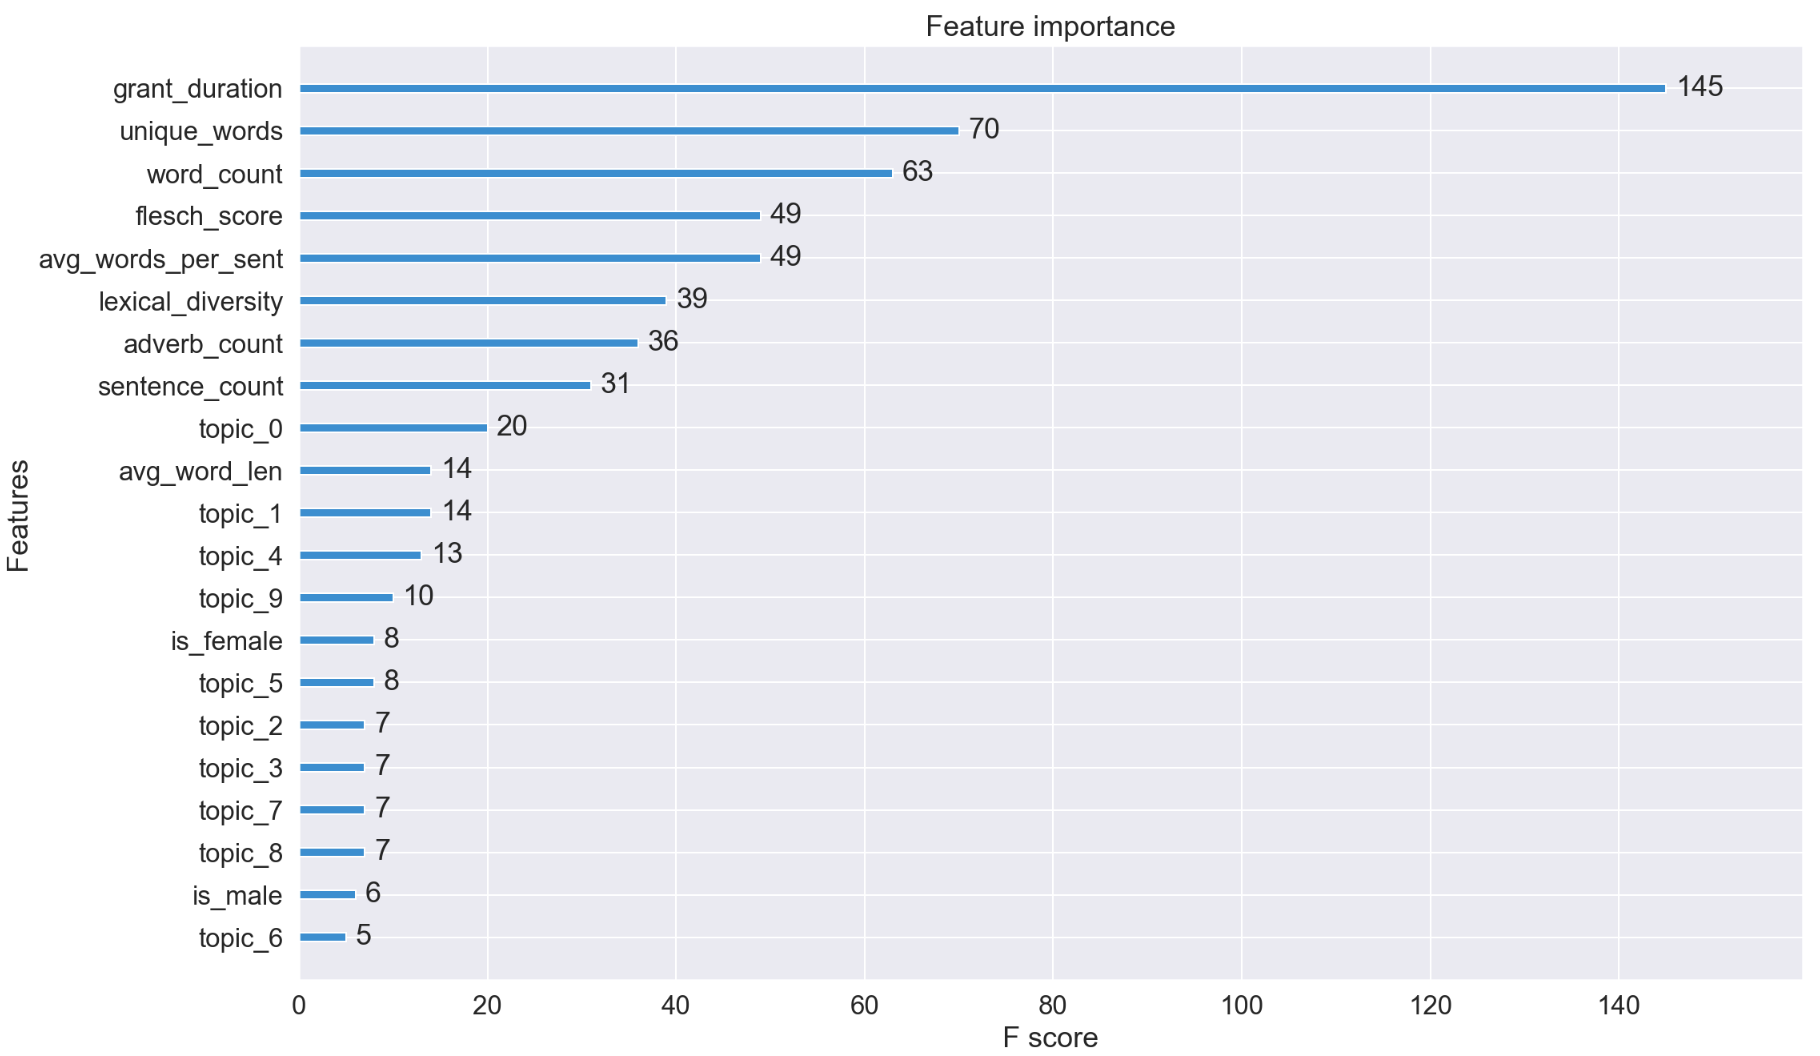
\includegraphics[width=\textwidth]{xgbLogAwardPerDay}
 
  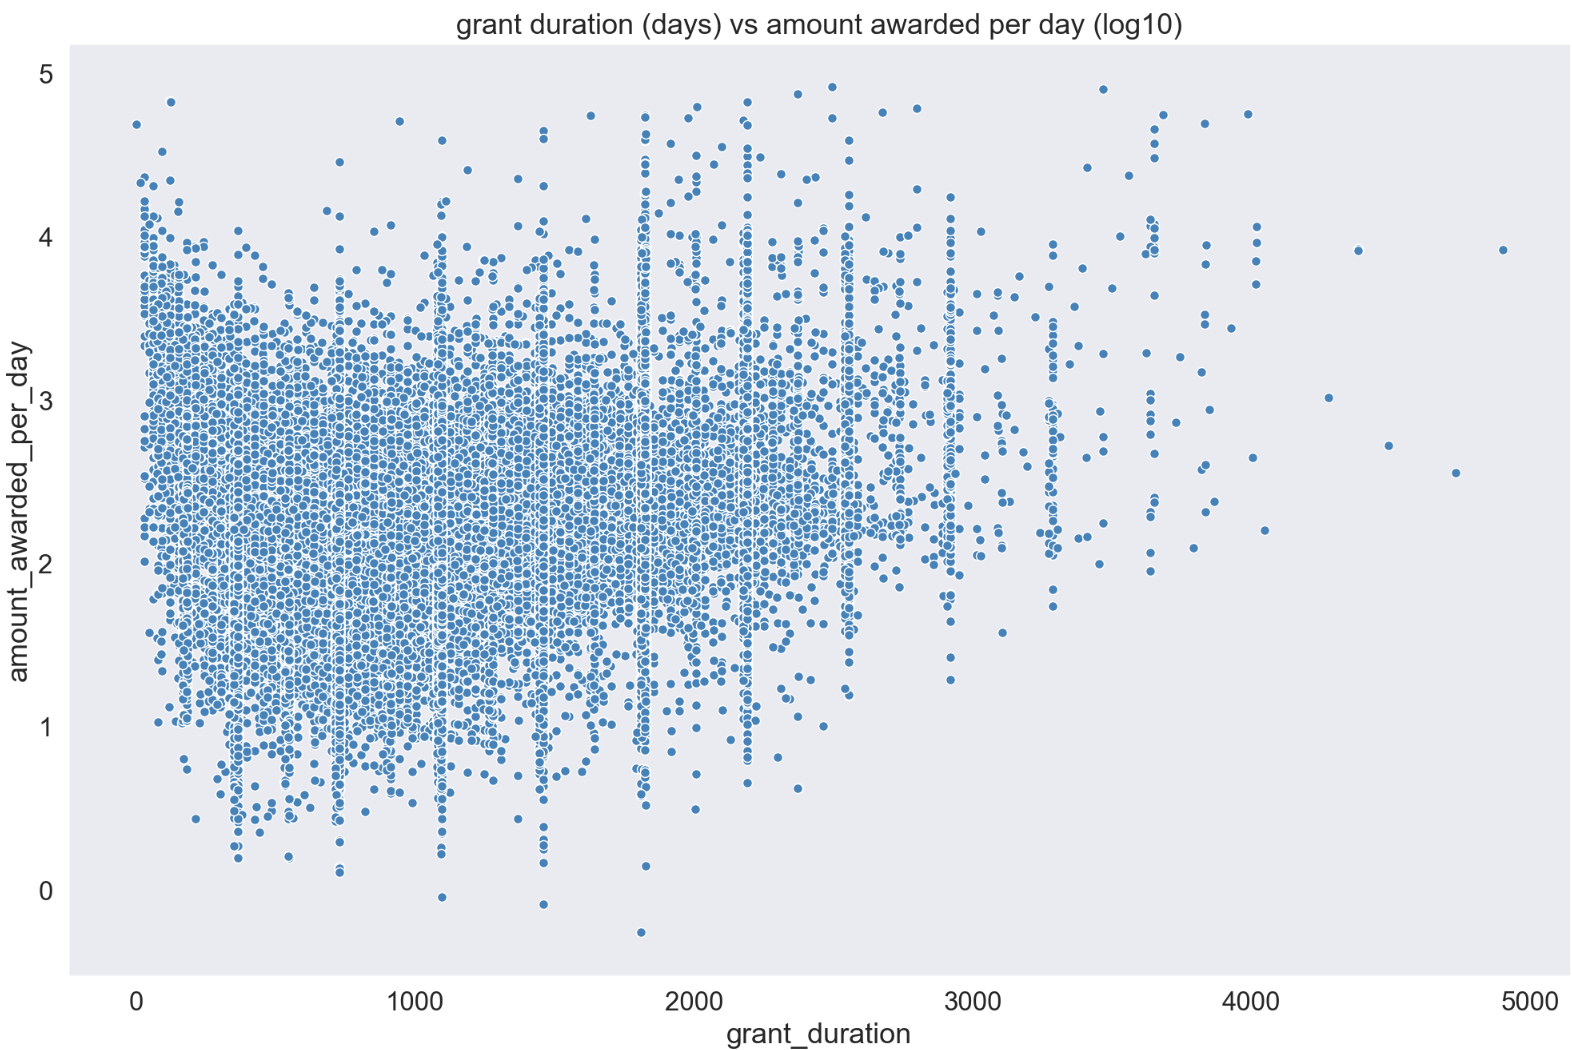
\includegraphics[width=\textwidth]{xgbScatterAwardPerDay}

A second model was trained using the \textbf{per day award amount without transformation}. The model shows that the second most important feature is the flesch ease score.

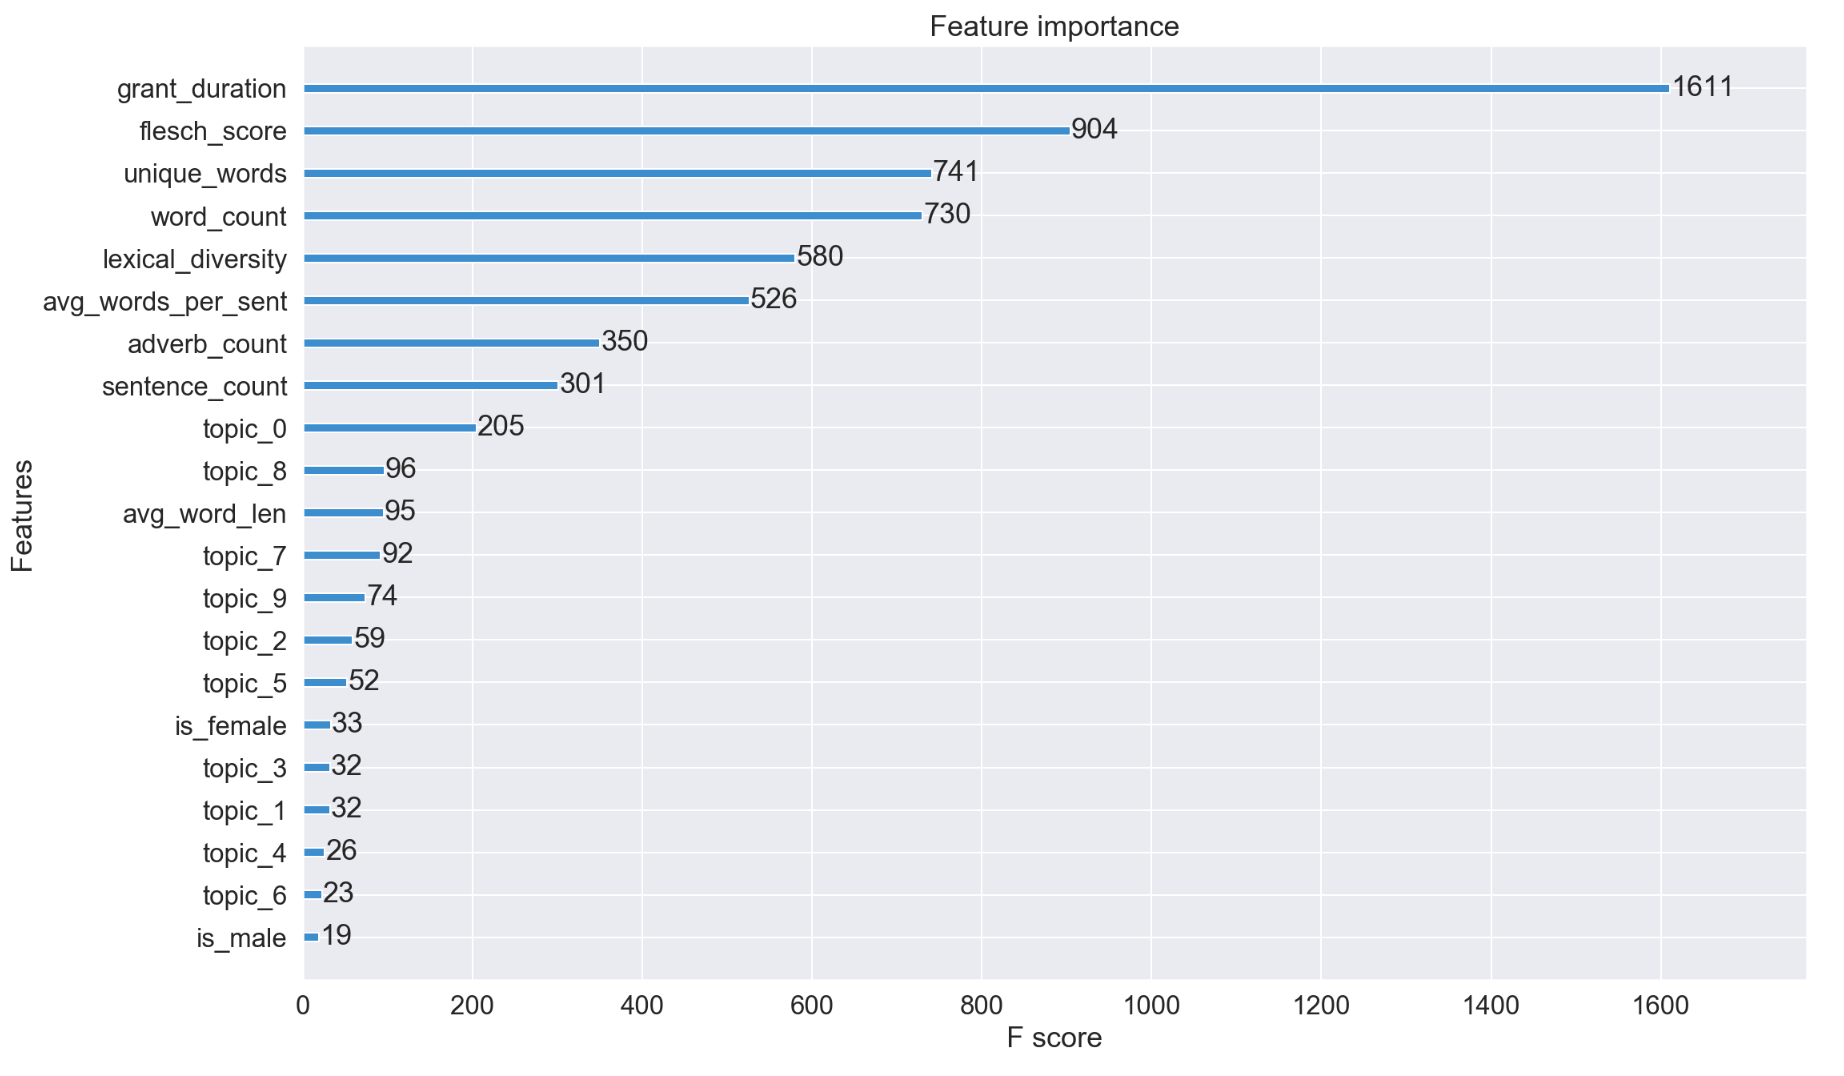
\includegraphics[width=\textwidth]{xgbAwardPerDay}

Most important features found using award per day with no log transformation as the target variable.

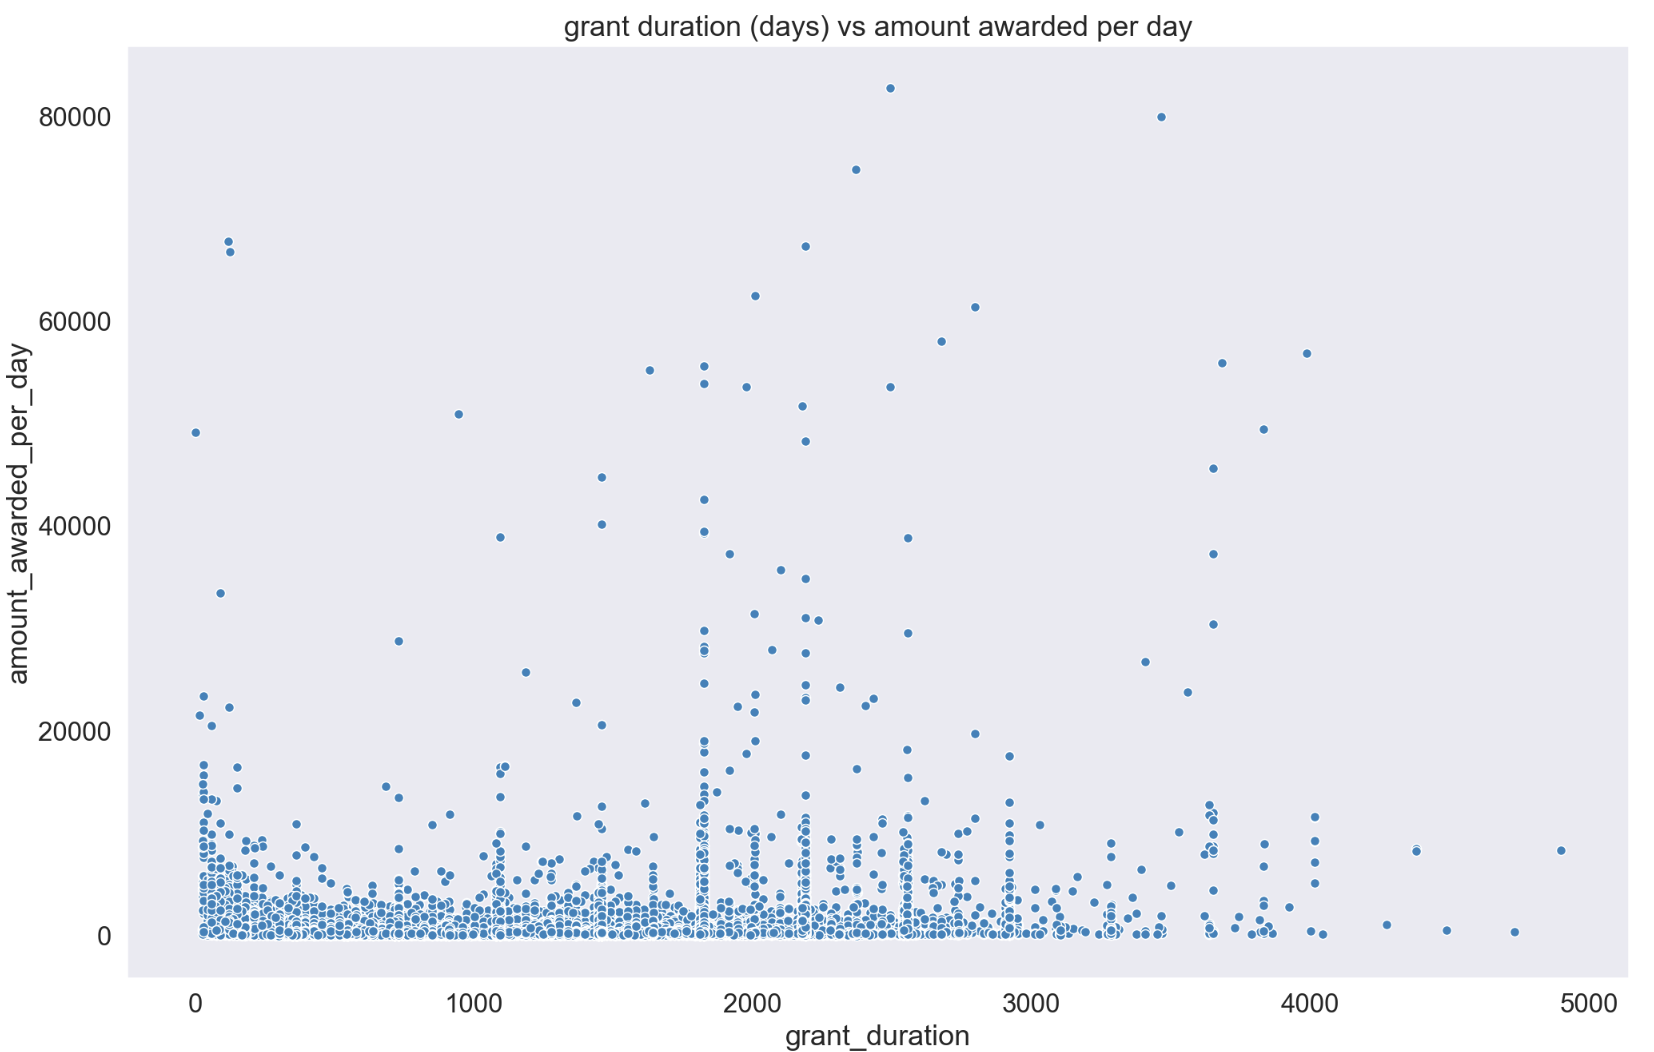
\includegraphics[width=\textwidth]{xgbScatterAwardPerDayNoLog}

 \textbf{ XGBoost model using award amount}
 
The following graphs shows the most important features found by the model using the total award amount as the target variable. Just like the previous models, grant duration is the most relevant feature.
 
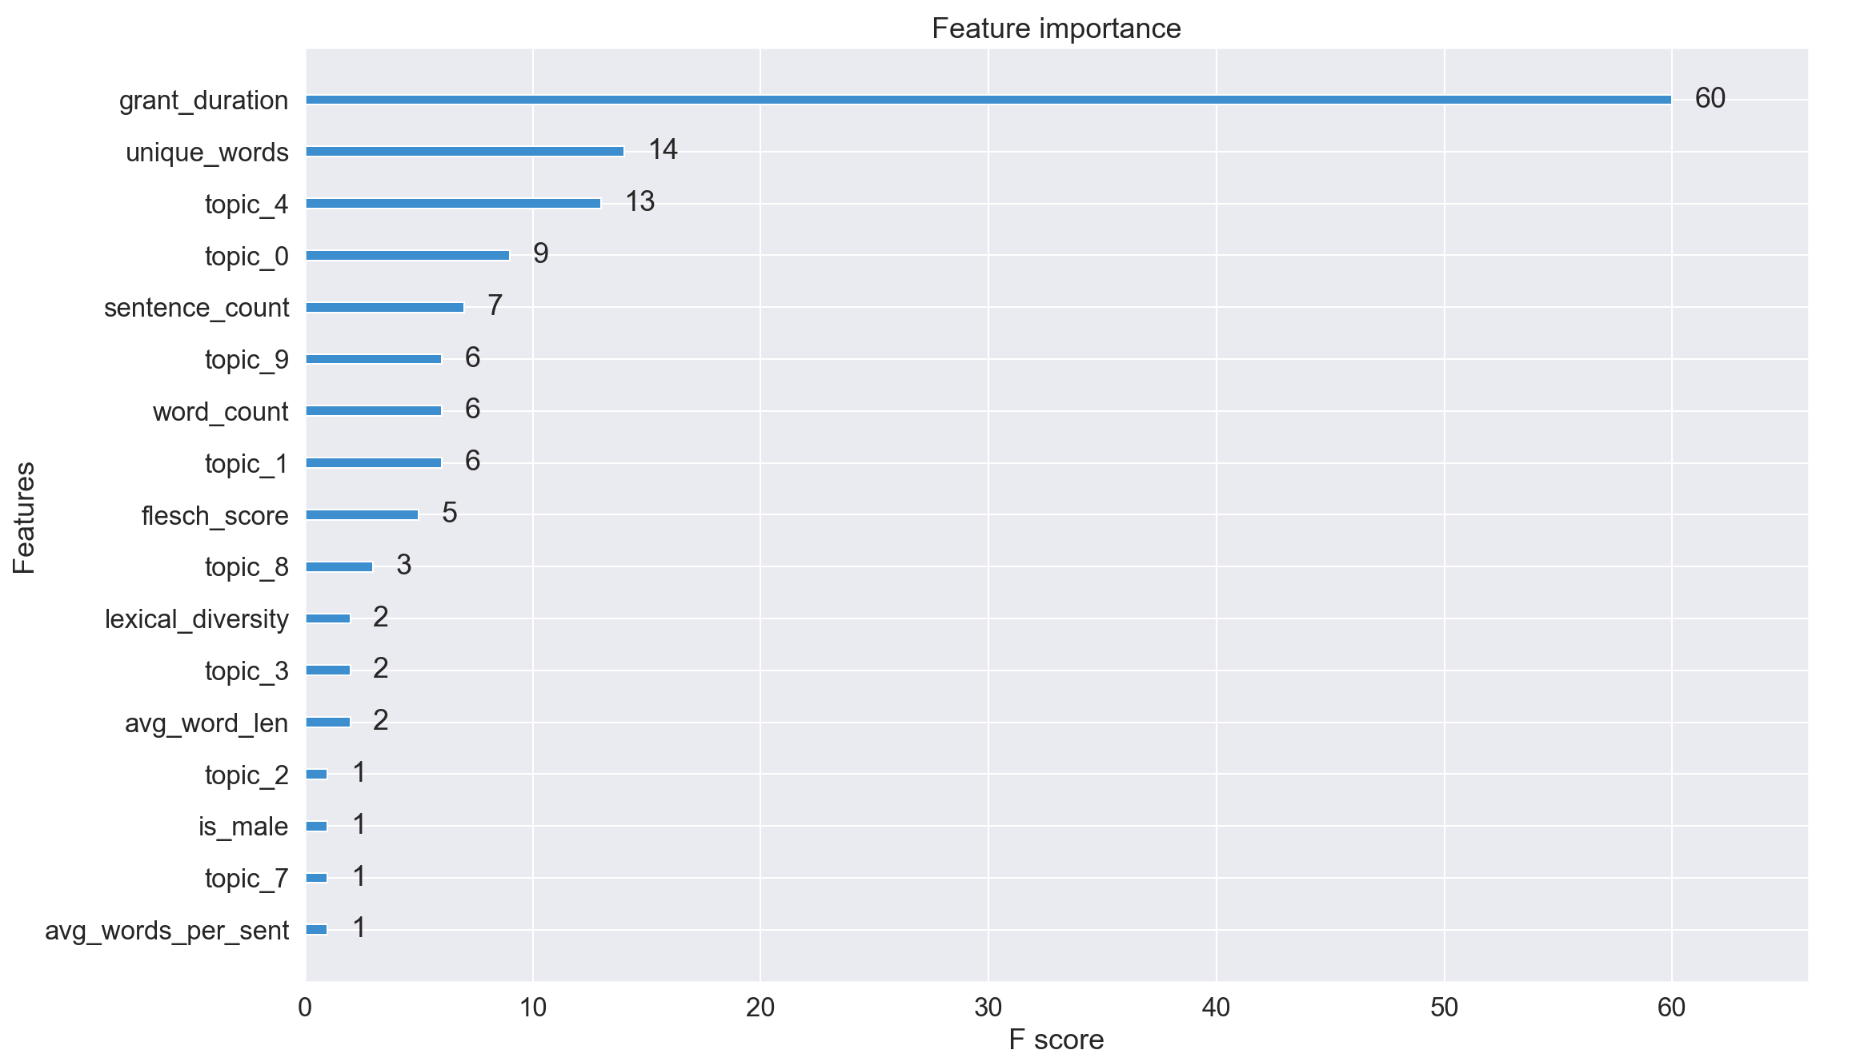
\includegraphics[width=\textwidth]{xgbAwardAmount}

The  following graph shows the linear relation of Grant duration in days and Award Amount.

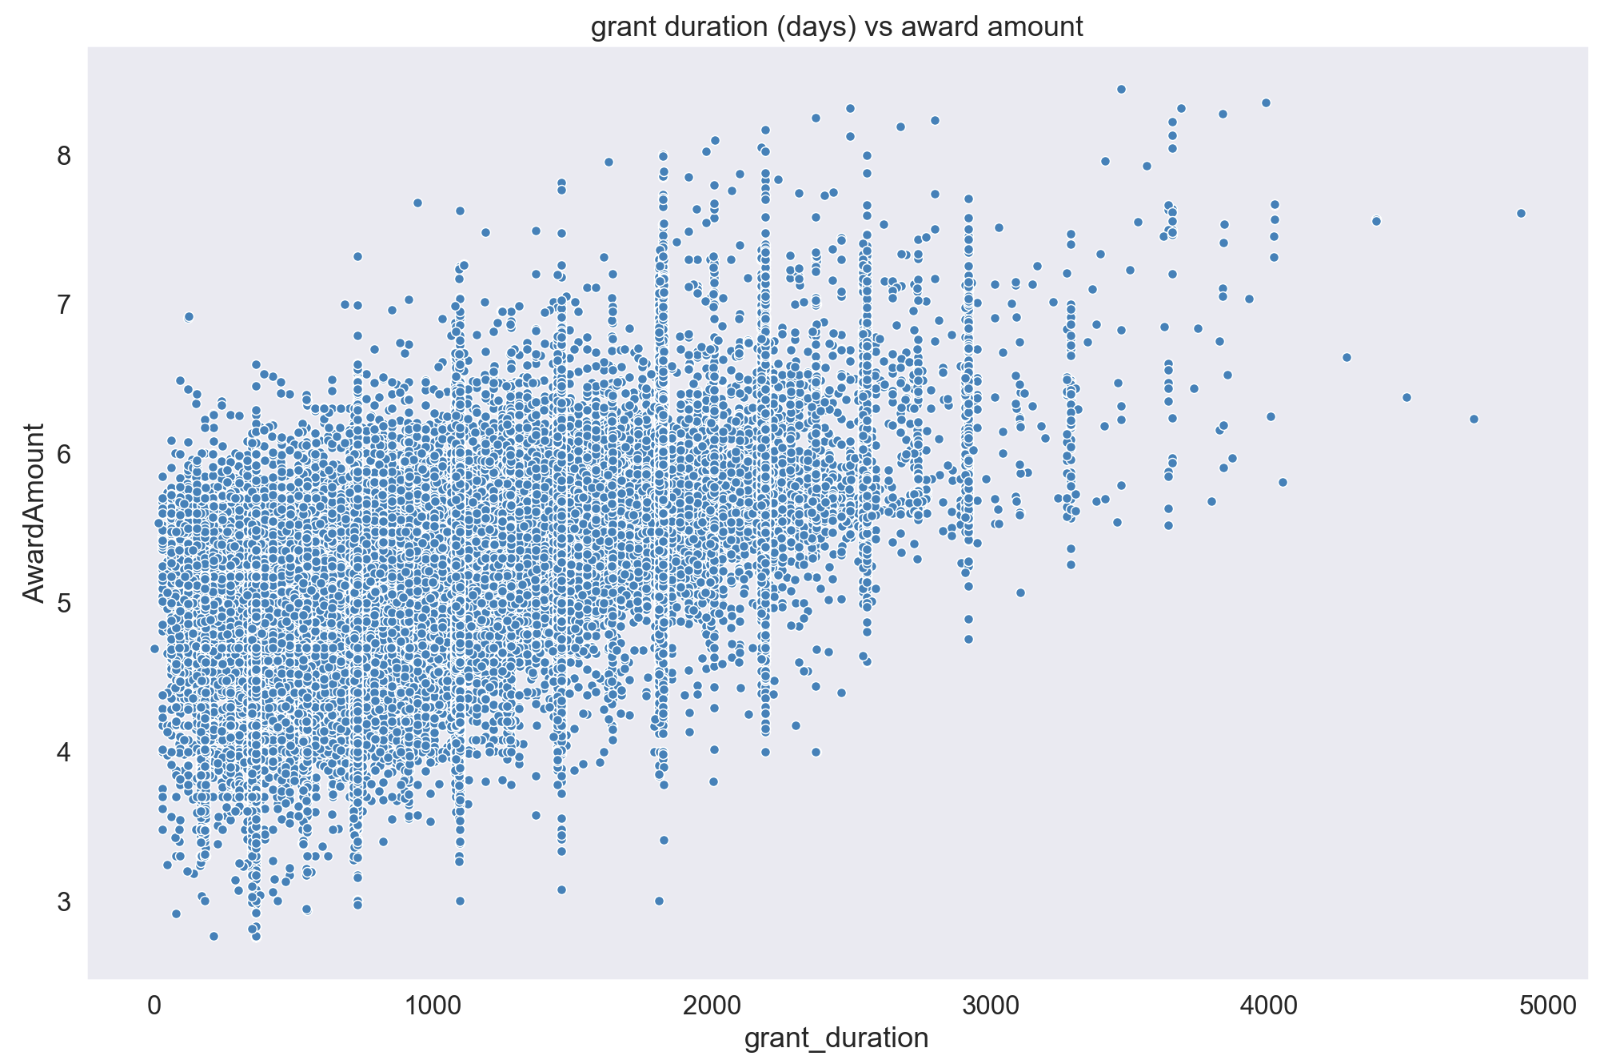
\includegraphics[width=\textwidth]{xgbScatterAwardAmount}

 \section{Conclusions} 
 
The previous analysis used data on projects funded by the NSF to conduct text analysis, topic modeling and create a predictive model to help identify whether language structure and project topic have an impact on the amount of money projects receive.

Since the hypothesis was that language patterns and abstract length had an impact on funding, feature engineering through text extraction was a key component to the analysis. The derived features, including gender of the program officer who approved the award, word count, unique word count, lexical complexity, grant duration, sentence count, average words per sentence, flesch ease read score and topic of the abstract provided relevant information to build the XGBoost models.

The results all the model used including gender classification, topic modeling and award amount prediction can be used not only to review project proposals submitted for NSF funding, but other U.S. government financial request.

 \section{Further Analysis}

Other features such as geographic location and name of the author or team who submitted the proposal could be used in further analysis to understand how research funding has been allocated throughout the U.S. over the years. Unfortunately for this analysis the geographic location attribute have a large number of missing values and there was no consistency in recording the name or institution of the author(s) of the proposal.

Additional feature engineering and different tuning parameters could also provide more relevant variables that can help predict the impact of language patterns in funding received.

\end{document}  